\section{Modelo de levitador magnético}

La ecuación mecánica para el sistema de levitación magnética ECP \cite{730} con el imán superior activado es:

\begin{equation}
m\ddot{x} = f_{\text{fld}}(i,x) - f_{\text{fr}} - mg
\label{eq:mec}
\end{equation}

Donde \( m \,[\text{kg}] \) es la masa, \( \ddot{x} \,[\text{m}/\text{s}^2] \) la aceleración,
 \( f_{\text{fld}} \,[\text{N}] \) la fuerza electromagnética, \( f_{\text{fr}} \,[\text{N}] \) la fuerza de fricción y \( mg \,[\text{N}] \) la fuerza gravitacional.

\section{\texorpdfstring{Formas de $f_{\text{fld}}$}{Formas de fld}}

Conciendo la forma de $L_{(x)}$ podemos determinar $f_{\text{fld}}$ por lo que la literatura científica se ha documentado la forma no lineal explicándola a través de una u otra . De acuerdo con Al-Muthair et al. \cite{al} cuando se levita un bola ferromagnética se puede aproximar como:

\[
f_{\text{fld}} = C\left(\dfrac{i}{x}\right)^2
\]

Donde $C$ es la constante de la fuerza magnética, $i$ la intensidad de la corriente eléctrica y $x$ la posición.

Charara et al. \cite{charara} calcula la fuerza electromagnética dentro de un conjinete como:

\[ 
f_{\text{fld}} = K\,\frac{\operatorname{sign}(i)\,i^{2}}{e^{2}}, 
\qquad \text{con } 
K = 0.25 \cos\!\left(\frac{\pi}{8}\right)\!\mu\, n^{2} S 
\]

Donde $S$ es el área de la cara del polo, $\mu$ es la permeabilidad magnética en el vacío y $n$ numero de vueltas del embobinado.

Según El Hajjaji et al. \cite{el} se determinó experimentalmente que la fuerza electromagnética sobre un esfera metálica tiene la forma:


\[ 
f_{\text{fld}} = \dfrac{i^{2}}{b_0 + b_1x + b_2x^3 + b_3x^4}
\]

con $b_0$= 0.0304, $b_1$ = 0.7159, $b_2$=-0.9165, $b_3$=1.1994 como parámetros del sistema


Zhao et al. \cite{zhao} calculan la fuerza del electroimán parar hacer levitar una bola metálica como:
\[ f_{\text{fld}} = \frac{L_0 x_0 i^2}{2x^2} \]

Donde $i$ es la corriente del embobinado, $x$ la posición de la bola, $L_0$ la inductancia del sistema en el punto de equilibrio $x_0$.

Feifie at al. \cite{feifei} de un sistema similar determina la fuerza electromagnética como:
\[ f_{\text{fld}} = \frac{K i^2}{(H - x)^2} \]

Donde $i$ es la intensidad de la corriente, $x$ la posición, $K$ y $H$ parámetros del sistema



Se puede apreciar que no hay un modelo único condicionado por la configuración del sistema y la metodología analítica o experimental que se empleó para modelarla. Por lo tanto se eligió 
el modelo del levitador ECP730 dado por el fabricante en su hoja de especificación técnica \cite{parks} y validada experimentalmente por Alcantara et al. \cite{alcantara} como:

\[ f_{\text{fld}} = \frac{u}{b(a-x)^4} \]

Donde $u$ es voltaje aplicado en las terminales del embobinado del electroimán, $x$ la posición del objeto levitante, $a$ y $b$ parámetros del sistema.

\section{Zona muerta dinámica no centrada en el origen}
Arturo \cite{arturo_tesis} sostiene que la zona muerta dura describe de manera más precisa el fenómeno observado en motores eléctricos, 
donde dicha no linealidad se manifiesta a partir $u_e{(t)} = 0$, el cual constituye el único voltaje de equilibrio en sistemas de control de posición angular.

En contraste, en los sistemas de levitación magnética existen múltiples voltajes de equilibrio, por lo que su representación matemática adopta la forma:

\[
v(t) = D\big(u(t)\big) =
\begin{cases}
m_r \big(u(t) - u_e - b_r\big) - h_r, & u(t) \ge b_r, \\[6pt]
0, & b_l < u(t) < b_r, \\[6pt]
m_l \big(u(t) - u_e - b_l\big) - h_l, & u(t) \le b_l.
\end{cases}
\]

Donde $m_r$, $b_r$, $h_r$, $m_l$, $b_l$ y $h_l$ son parámetros desconocidos de la zona muerta, pero de signos conocidos:
$m_r > 0$, $m_l > 0$, $b_r > 0$, $b_l < 0$, $h_r < 0$, $h_l > 0$

\section{Efecto atascamiento-deslizamiento}
El fenómeno de atascamiento-deslizamiento es característico de los sistemas con fricción, donde el movimiento no transcurre de forma continua y gradual sino más bien donde ocurre alternancia de atascamiento(ausencia de movimiento) y deslizamiento (movimiento repentino). 
Los modelos de fricción que se han documentado tratan de modelar este comportamiento \cite{armstrong,olsson,berman}. Se considera un modelo de fricción compuesto que permite considerar para $v = 0$ el sistema se encuentra en régimen de fricción estática; si la fuerza externa aplicada al sistema entra en movimiento pasa a régimen de fricción dinámica debido al descenso repentino del valor de fricción, la intermitencia 
entre estás etapas es lo que se conoce como efecto atascamiento-deslizamiento. 

\[
f_{\text{fric}} =
\begin{cases}
c\,v, 
& v \neq 0, \\[6pt]

\min\!\left(|F_e|,\,F_s\right)\,\operatorname{sign}(F_e),
& v = 0
\end{cases}
\]


donde $f_{\text{fric}}$ es la fuerza de fricción, $F_{e}(t)$ es la fuerza externa,
$F_{s}$ es la fricción estática máxima,
$c$ es el coeficiente de fricción viscosa y $v$ es la velocidad relativa.

La forma en que se hacen estas transciones entre régimes se presenta de manera regular induciendo la formación de ciclos límite. 



El modelo completo del sistema 
\begin{figure}[h]
    \centering
       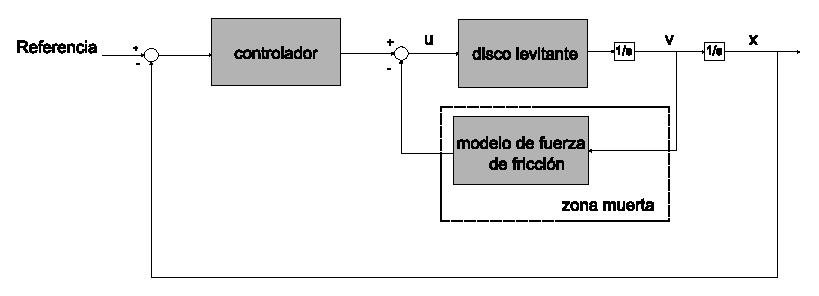
\includegraphics[width=0.6\textwidth]{images/chapter_1/lazo_de_control_con_zm.eps}
    \caption{Lazo de control con zona muerta}
    \label{lazo_de_control_con_zm}
\end{figure}

\section{Soluciones numéricas}
El efecto atascamiento-deslizamiento por la fricción es difícil de simular en el diseño de controladores con retroalimentación para sistemas con componente mecánico dado 
por el comportamiento no lineal alrededor de la velocidad cero, en este punto se convierte en un problema numérico más que físico, 
de hecho existe una amplia variedad de estrategias que modelan e implementan este fenómeno, conocidos como modelos dinámicos de fricción \cite{haessig}.

El método de Karnopp\cite{karnopp} introduce una banda de velocidad $\left| DV \right|$ donde se considera la velocidad cero y por tanto decidir cuando el sistema esta atascado o en deslizamiento; por su fácil implementación
permite que se emplee en aplicaciones prácticas para el diseño de actuadores \cite{liu}\cite{ravanbod}\cite{ravanbod1}\cite{bicakci}\cite{romano}; por ello, se utiliza en las simulaciones.

\section{Modelo linealizado sistema de levitación magnética}
Los parámetros del modelo no lineal ($a$, $b$, $c_1$, $m$, $g$) fueron identificados experimentalmente por Alcántara et al.\ \cite{diana_tesis} para el dispositivo ECP-730 en configuración repulsiva (estable en lazo abierto), mediante ensayos de estado estacionario y respuesta dinámica en lazo abierto. En el presente trabajo se adoptan esos mismos parámetros y se aplican a la configuración atractiva (inestable en lazo abierto), en la que la bobina superior atrae al imán levitante. Si bien la estructura funcional del modelo es idéntica, en la configuración atractiva la fuerza magnética crece al disminuir la brecha entre el imán y la bobina, lo que hace que los puntos de equilibrio sean inestables. El modelo linealizado en representación en espacio de estados para la configuración inestable queda como:
\[
\begin{aligned}
\dot{x}
&=
\begin{bmatrix}
0 & 1 \\[6pt]
\dfrac{4g}{(a-x_1^{\ast})} & -c_1
\end{bmatrix}x
+
\begin{bmatrix}
0 \\[6pt]
\dfrac{1}{mb\,(a-x_1^{\ast})^4}
\end{bmatrix}u,
\\[10pt]
y &= \begin{bmatrix} 1 & 0 \end{bmatrix} x
\end{aligned}
\]


Donde la posición $x_1$ y la velocidad $x_2$ forman el vector de estado $x$, $y$ el vector de salida, $c_1$ el coeficiente de fricción viscosa por unidad de masa y $x_1^{\ast}$ siendo el valor de posición donde se alcanza el punto de equilibrio.

La ecuación característica queda como:

\[
\lambda^2 + c_1\lambda - \dfrac{4g}{(a-x_1^{\ast})} = 0
\]

Como $a - x_1^{\ast} > 0$ para toda posición alcanzable, el término independiente es negativo y la ecuación característica tiene siempre una raíz real positiva: todos los puntos de equilibrio de la configuración atractiva son inestables. En $x_1^{\ast}=-4$~cm las raíces son $\lambda_1 = -23{,}5057$ y $\lambda_2 = 14{,}9427$.

Se verifica que el sistema es controlable y observable

\[
\mathcal{C}
=
\begin{bmatrix}
0 & b_0\\[6pt]
b_0 & -c_1 b_0
\end{bmatrix}
\qquad
\mathcal{O}
=
\begin{bmatrix}
1 & 0\\[6pt]
0 & 1
\end{bmatrix}
\]

Donde $b_0 = \dfrac{1}{m\,b\,(a-x_1^{\ast})^4}$. Ambas matrices son linealmente independientes, por tanto con la señal de entrada de la planta se modifica su espacio de estados y de su salida se
deduce en que punto dentro del estado espacio de estados se encuentra la planta.
Los valores paramétricos de $c_1$, $b$, $a$, $m$ y $g$ que se emplearon para realizar los cálculos fueron identificados experimentalmente por Alcántara et al.\ \cite{diana_tesis}; se reúnen en la tabla~\ref{tab:parametros} junto con los parámetros del modelo de fricción y el intervalo de la señal de control. Las fuerzas se expresan en $\text{kg}\cdot\text{cm}/\text{s}^2$, unidades en las que el peso del imán es $mg = 138{,}3$. En \cite{diana_tesis}, $c_1$ se reporta en $\text{kg}^{-1}$; dado que multiplica a la velocidad en la ecuación de aceleración, sus unidades consistentes son $\text{s}^{-1}$.

\begin{table}[h]
\centering
\caption{Parámetros del modelo}
\label{tab:parametros}
\begin{tabular}{|c|c|l|}
\hline
$a$ & $7.17184\;[\text{cm}]$ & parámetro de la fuerza electromagnética \\ \hline
$b$ & $1.6163 \times 10^{-6}\;[\text{V}/(\text{N}\cdot\text{cm}^4)]$ & parámetro de la fuerza electromagnética \\ \hline
$c_1$ & $8.563\;[\text{s}^{-1}]$ & fricción viscosa por unidad de masa \\ \hline
$m$ & $0.141\;[\text{kg}]$ & masa del imán levitante \\ \hline
$g$ & $981\;[\text{cm}/\text{s}^2]$ & aceleración de la gravedad \\ \hline
$F_s$ & $20\;[\text{kg}\cdot\text{cm}/\text{s}^2]$ ($0.2$~N) & fricción estática máxima (Karnopp) \\ \hline
$DV$ & $0.02\;[\text{cm}/\text{s}]$ & banda de velocidad nula (Karnopp) \\ \hline
$u$ & $[0,\ 3.5]\;[\text{V}]$ & intervalo de la señal de control \\ \hline
\end{tabular}
\end{table}


% Generado a partir de calculus/Final_Bien/evidencia_P8.m (simulador corregido).
\subsection{Sistema no lineal en lazo abierto en los puntos de equilibrio}

Para caracterizar la inestabilidad de la configuración atractiva, se simuló el modelo no lineal sin fricción estática ni zona muerta, aplicando el voltaje de equilibrio $u=u_e(x_1^*)$ y desplazando la posición inicial $0{,}01$~cm respecto al equilibrio, en $x_1^*=-4$, $-3$ y $-2$~cm. La figura~\ref{fig:p8_lazo_abierto} muestra que la desviación crece exponencialmente y alcanza 1~cm en $0{,}33$, $0{,}32$ y $0{,}30$~s, respectivamente; el modelo linealizado reproduce el crecimiento con un tiempo de duplicación $\ln 2/\lambda_2$ de $46$, $44$ y $41$~ms. Cuanto más cerca de la bobina se encuentra el equilibrio, más rápido es el polo inestable.

\begin{figure}[ht]
    \centering
    % Estilo común de las figuras de evidencia P8 (pgfplots).
\pgfplotsset{
  pocho/.style={
    width=0.92\textwidth, height=5.2cm,
    grid=major, grid style={gray!25},
    tick label style={font=\small}, label style={font=\small}, legend style={font=\small},
    /pgf/number format/use comma,
    scaled ticks=false,
    y tick label style={/pgf/number format/fixed},
    table/col sep=comma, unbounded coords=jump,
    every axis plot/.append style={line join=round},
  },
}
\definecolor{tray}{RGB}{31,94,166}
\definecolor{refc}{RGB}{40,40,40}
\definecolor{ctl2}{RGB}{196,96,40}
\definecolor{ver}{RGB}{46,133,64}

\begin{tikzpicture}
\begin{semilogyaxis}[pocho, height=6cm, xmin=0, xmax=0.36, ymin=0.01, ymax=1,
    xlabel={tiempo [\si{s}]}, ylabel={$|x_1(t)-x_1^*|$ [\si{cm}]},
    x tick label style={/pgf/number format/fixed},
    legend style={at={(0.02,0.98)}, anchor=north west}, legend cell align=left]
  \addplot[tray, line width=1pt]  table[x=t, y=nl_m4] {images/p8_results/tikz/lazo_abierto.csv}; \addlegendentry{$x_1^*=-4$ cm}
  \addplot[ctl2, line width=1pt]  table[x=t, y=nl_m3] {images/p8_results/tikz/lazo_abierto.csv}; \addlegendentry{$x_1^*=-3$ cm}
  \addplot[ver, line width=1pt]   table[x=t, y=nl_m2] {images/p8_results/tikz/lazo_abierto.csv}; \addlegendentry{$x_1^*=-2$ cm}
  \addplot[tray, densely dashed]  table[x=t, y=lin_m4] {images/p8_results/tikz/lazo_abierto.csv}; \addlegendentry{modelo lineal}
  \addplot[ctl2, densely dashed, forget plot] table[x=t, y=lin_m3] {images/p8_results/tikz/lazo_abierto.csv};
  \addplot[ver, densely dashed, forget plot]  table[x=t, y=lin_m2] {images/p8_results/tikz/lazo_abierto.csv};
\end{semilogyaxis}
\end{tikzpicture}

    \caption[Lazo abierto en los puntos de equilibrio]{Desviación respecto al equilibrio en lazo abierto, con $u=u_e$ y una perturbación inicial de $0{,}01$~cm. Líneas continuas: modelo no lineal; discontinuas: modelo linealizado.}
    \label{fig:p8_lazo_abierto}
\end{figure}

El retrato de fase alrededor de $x_1^*=-4$~cm (figura~\ref{fig:p8_retrato}) confirma que el equilibrio es un punto silla: las trayectorias se alejan a lo largo de la variedad inestable, salvo las que parten exactamente sobre la variedad estable. Al incorporar la fricción estática de Karnopp cambia la situación en reposo: si el levitante está detenido y $u=u_e$, la fuerza neta $u/[b(a-x)^4]-mg$ no supera $F_s$ mientras la posición se encuentre entre $-4{,}44$ y $-3{,}63$~cm, de modo que el imán permanece atascado en cualquier punto de esa banda. Para $x_1^*=-3$ y $-2$~cm las bandas correspondientes son $[-3{,}41;\,-2{,}66]$ y $[-2{,}37;\,-1{,}70]$~cm. La fricción estática enmascara así la inestabilidad del equilibrio mientras el levitante no se mueva.

\begin{figure}[ht]
    \centering
    % Estilo común de las figuras de evidencia P8 (pgfplots).
\pgfplotsset{
  pocho/.style={
    width=0.92\textwidth, height=5.2cm,
    grid=major, grid style={gray!25},
    tick label style={font=\small}, label style={font=\small}, legend style={font=\small},
    /pgf/number format/use comma,
    scaled ticks=false,
    y tick label style={/pgf/number format/fixed},
    table/col sep=comma, unbounded coords=jump,
    every axis plot/.append style={line join=round},
  },
}
\definecolor{tray}{RGB}{31,94,166}
\definecolor{refc}{RGB}{40,40,40}
\definecolor{ctl2}{RGB}{196,96,40}
\definecolor{ver}{RGB}{46,133,64}

\begin{tikzpicture}
\begin{axis}[pocho, width=0.8\textwidth, height=7.5cm, xmin=-4.5, xmax=-3.5, ymin=-10, ymax=10,
    xlabel={posición $x_1$ [\si{cm}]}, ylabel={velocidad $x_2$ [\si{cm/s}]},
    legend style={at={(0.98,0.02)}, anchor=south east, fill=white}, legend cell align=left]
  \addplot[gray!60, quiver={u=\thisrow{dx}, v=\thisrow{dv}, every arrow/.append style={-stealth}}, forget plot]
    table[x=x, y=v] {images/p8_results/tikz/campo.csv};
  \addplot[tray, line width=0.9pt] table[x=x, y=v] {images/p8_results/tikz/trayectorias.csv}; \addlegendentry{trayectorias}
  \addplot[ctl2, line width=1.4pt] table[x=x, y=v] {images/p8_results/tikz/variedad_inestable.csv}; \addlegendentry{variedad inestable}
  \addplot[ver, line width=3pt, opacity=0.6] coordinates {(-4.4448,0) (-3.6291,0)}; \addlegendentry{banda de atascamiento ($u=u_e$)}
  \addplot[only marks, mark=*, mark size=2pt, refc] coordinates {(-4,0)}; \addlegendentry{equilibrio $x_1^*=-4$ cm}
\end{axis}
\end{tikzpicture}

    \caption[Retrato de fase en lazo abierto]{Retrato de fase del modelo no lineal sin fricción estática alrededor de $x_1^*=-4$~cm, con $u=u_e$. La banda verde indica las posiciones en las que, con el levitante en reposo, la fricción estática lo mantiene atascado.}
    \label{fig:p8_retrato}
\end{figure}

\FloatBarrier


\subsection{Control con doble efecto integral}
Se diseñó un controlador con PII que permita reducir el tiempo de atascamiento del sistema en comparación con el PI, quedando como:

\[
C(s)=\frac{152.43\,(s+4.875)(s+1.861)(s+17.31)}
{s^{2}(s+301.1)}
\]

\begin{figure}[ht]
    \centering
    % Estilo común de las figuras de diseño del PII (pgfplots).
% Generado por diseno_PII_tikz.m
\def\PIIwg{9.6320}
\def\PIImgwg{17.0713}
\def\PIIwp{129.2942}
\def\PIIphwp{-120.1396}
\def\PIIgmdb{-17.1}
\def\PIIpm{59.9}
\def\PIIos{16.9}
\def\PIIts{0.284}
\def\PIItp{0.0238}
\def\PIIyp{1.1688}
\def\PIIflechaA{(-7.6265,1.7150) -- (-7.5765,1.4566)}
\def\PIIflechaC{(-7.5765,-1.4566) -- (-7.6265,-1.7150)}
\def\PIIflechaB{(-2.6114,-3.2049) -- (-2.5176,-3.1809)}
\def\PIIflechaD{(-2.5176,3.1809) -- (-2.6114,3.2049)}

\pgfplotsset{
  diseno/.style={
    grid=major, grid style={gray!25},
    tick label style={font=\small}, label style={font=\small}, legend style={font=\small},
    /pgf/number format/use comma,
    table/col sep=comma,
    every axis plot/.append style={line join=round},
  },
}
\definecolor{tray}{RGB}{31,94,166}
\definecolor{marg}{RGB}{196,96,40}
\definecolor{refc}{RGB}{40,40,40}

\begin{tikzpicture}
\begin{axis}[diseno, name=mag, width=0.85\textwidth, height=5.2cm, xmode=log,
             xmin=1e-2, xmax=1e4, ymin=-100, ymax=110, ytick={-100,-50,0,50,100},
             xticklabels={}, ylabel={magnitud [\si{dB}]}]
  \addplot[refc!50, densely dashed] coordinates {(1e-2,0) (1e4,0)};
  \addplot[tray, line width=1pt] table[x=w, y=mag_db] {images/pii_design/tikz/bode.csv};
  \draw[marg, line width=0.8pt] (axis cs:\PIIwg,0) -- (axis cs:\PIIwg,\PIImgwg);
  \addplot[marg, only marks, mark=*, mark size=1.8pt] coordinates {(\PIIwg,\PIImgwg)};
  \node[font=\small, anchor=north east, align=left, fill=white, inner sep=2pt]
    at (axis cs:8e3,104) {MG $=\num{\PIIgmdb}$~\si{dB} en $\omega=\num[round-mode=places,round-precision=2]{\PIIwg}$~\si{rad/s}};
\end{axis}
\begin{axis}[diseno, at={(mag.south west)}, anchor=north west, yshift=-0.35cm,
             width=0.85\textwidth, height=5.2cm, xmode=log,
             xmin=1e-2, xmax=1e4, ymin=-375, ymax=-90, ytick={-360,-315,-270,-225,-180,-135},
             xlabel={frecuencia [\si{rad/s}]}, ylabel={fase [\si{\degree}]}]
  \addplot[refc!50, densely dashed] coordinates {(1e-2,-180) (1e4,-180)};
  \addplot[tray, line width=1pt] table[x=w, y=fase] {images/pii_design/tikz/bode.csv};
  \draw[marg, line width=0.8pt] (axis cs:\PIIwp,-180) -- (axis cs:\PIIwp,\PIIphwp);
  \addplot[marg, only marks, mark=*, mark size=1.8pt] coordinates {(\PIIwp,\PIIphwp)};
  \node[font=\small, anchor=south east, align=left, fill=white, inner sep=2pt]
    at (axis cs:8e3,-370) {MF $=\num{\PIIpm}\si{\degree}$ en $\omega=\num[round-mode=places,round-precision=1]{\PIIwp}$~\si{rad/s}};
\end{axis}
\end{tikzpicture}

    \caption[Diagrama de Bode]{Diagrama de Bode del lazo abierto $L(s)=C(s)G(s)$ en $x_1^*=-4$~cm. Se indican el margen de ganancia (inferior, por el polo inestable de la planta) y el margen de fase.}
    \label{bode_fase}
\end{figure}

\begin{figure}[ht]
    \centering
    % Estilo común de las figuras de diseño del PII (pgfplots).
% Generado por diseno_PII_tikz.m
\def\PIIwg{9.6320}
\def\PIImgwg{17.0713}
\def\PIIwp{129.2942}
\def\PIIphwp{-120.1396}
\def\PIIgmdb{-17.1}
\def\PIIpm{59.9}
\def\PIIos{16.9}
\def\PIIts{0.284}
\def\PIItp{0.0238}
\def\PIIyp{1.1688}
\def\PIIflechaA{(-7.6265,1.7150) -- (-7.5765,1.4566)}
\def\PIIflechaC{(-7.5765,-1.4566) -- (-7.6265,-1.7150)}
\def\PIIflechaB{(-2.6114,-3.2049) -- (-2.5176,-3.1809)}
\def\PIIflechaD{(-2.5176,3.1809) -- (-2.6114,3.2049)}

\pgfplotsset{
  diseno/.style={
    grid=major, grid style={gray!25},
    tick label style={font=\small}, label style={font=\small}, legend style={font=\small},
    /pgf/number format/use comma,
    table/col sep=comma,
    every axis plot/.append style={line join=round},
  },
}
\definecolor{tray}{RGB}{31,94,166}
\definecolor{marg}{RGB}{196,96,40}
\definecolor{refc}{RGB}{40,40,40}

\begin{tikzpicture}
\begin{axis}[diseno, width=0.8\textwidth, height=0.62\textwidth,
             xmin=-10, xmax=2, ymin=-7, ymax=7, axis equal image,
             xlabel={$\operatorname{Re}\{L(j\omega)\}$}, ylabel={$\operatorname{Im}\{L(j\omega)\}$},
             legend pos=north west, legend cell align=left]
  \addplot[refc!40, thin, forget plot] coordinates {(-10,0) (2,0)};
  \addplot[refc!40, thin, forget plot] coordinates {(0,-7) (0,7)};
  \addplot[refc!55, densely dashed, domain=0:360, samples=120, forget plot] ({cos(x)},{sin(x)});
  \addplot[tray, line width=1pt]
    table[x=re, y=im] {images/pii_design/tikz/nyquist_pos.csv};
  \addlegendentry{$\omega>0$}
  \addplot[tray!55, line width=0.8pt, densely dashed]
    table[x=re, y=im] {images/pii_design/tikz/nyquist_neg.csv};
  \addlegendentry{$\omega<0$}
  \addplot[red!75!black, only marks, mark=+, mark size=4pt, line width=1.2pt] coordinates {(-1,0)};
  \addlegendentry{$-1$}
  \draw[tray, -stealth, line width=1pt] \PIIflechaA;
  \draw[tray, -stealth, line width=1pt] \PIIflechaB;
  \draw[tray!55, -stealth, line width=0.8pt] \PIIflechaC;
  \draw[tray!55, -stealth, line width=0.8pt] \PIIflechaD;
  \draw[marg, thin] (axis cs:-7.14,0) -- (axis cs:-8.5,-1.2);
  \node[font=\small, anchor=north, fill=white, inner sep=1.5pt] at (axis cs:-8.5,-1.2) {$-1/\mathrm{MG}$};
  \addplot[marg, only marks, mark=*, mark size=1.6pt, forget plot] coordinates {(-7.14,0)};
\end{axis}
\end{tikzpicture}

    \caption[Diagrama de Nyquist]{Diagrama de Nyquist de $L(s)$. Con un polo de lazo abierto en el semiplano derecho ($P=1$), la estabilidad en lazo cerrado exige un rodeo antihorario al punto $-1$.}
    \label{nyquist}
\end{figure}

\begin{figure}[ht]
    \centering
    % Estilo común de las figuras de diseño del PII (pgfplots).
% Generado por diseno_PII_tikz.m
\def\PIIwg{9.6320}
\def\PIImgwg{17.0713}
\def\PIIwp{129.2942}
\def\PIIphwp{-120.1396}
\def\PIIgmdb{-17.1}
\def\PIIpm{59.9}
\def\PIIos{16.9}
\def\PIIts{0.284}
\def\PIItp{0.0238}
\def\PIIyp{1.1688}
\def\PIIflechaA{(-7.6265,1.7150) -- (-7.5765,1.4566)}
\def\PIIflechaC{(-7.5765,-1.4566) -- (-7.6265,-1.7150)}
\def\PIIflechaB{(-2.6114,-3.2049) -- (-2.5176,-3.1809)}
\def\PIIflechaD{(-2.5176,3.1809) -- (-2.6114,3.2049)}

\pgfplotsset{
  diseno/.style={
    grid=major, grid style={gray!25},
    tick label style={font=\small}, label style={font=\small}, legend style={font=\small},
    /pgf/number format/use comma,
    table/col sep=comma,
    every axis plot/.append style={line join=round},
  },
}
\definecolor{tray}{RGB}{31,94,166}
\definecolor{marg}{RGB}{196,96,40}
\definecolor{refc}{RGB}{40,40,40}

\begin{tikzpicture}
\begin{axis}[diseno, width=0.85\textwidth, height=6cm, xmin=0, xmax=0.6, ymin=0, ymax=1.32,
             xlabel={tiempo [\si{s}]}, ylabel={amplitud},
             xtick={0,0.1,...,0.6}, x tick label style={/pgf/number format/fixed}]
  \addplot[refc!55, densely dashed] coordinates {(0,1) (0.6,1)};
  \addplot[refc!30, densely dotted, forget plot] coordinates {(0,0.98) (0.6,0.98)};
  \addplot[refc!30, densely dotted, forget plot] coordinates {(0,1.02) (0.6,1.02)};
  \addplot[tray, line width=1pt] table[x=t, y=y] {images/pii_design/tikz/escalon.csv};
  \addplot[marg, only marks, mark=*, mark size=1.8pt] coordinates {(\PIItp,\PIIyp)};
  \node[font=\small, anchor=south west, inner sep=2pt] at (axis cs:\PIItp,\PIIyp)
    {sobrepaso \SI{\PIIos}{\percent}};
  \draw[marg, densely dashed] (axis cs:\PIIts,0) -- (axis cs:\PIIts,0.98);
  \node[font=\small, anchor=south west, fill=white, inner sep=2pt] at (axis cs:\PIIts,0.08)
    {$t_s=\num{\PIIts}$~\si{s} (\SI{2}{\percent})};
\end{axis}
\end{tikzpicture}

    \caption[Respuesta al escalón]{Respuesta al escalón unitario del lazo cerrado linealizado.}
    \label{step_response}
\end{figure}    

\FloatBarrier
\newpage

% Generado a partir de calculus/Final_Bien/evidencia_P8.m (simulador corregido).
\subsection{Controlador con atascamiento-deslizamiento sobre el modelo lineal}

Para separar el efecto de las no linealidades no suaves del de la no linealidad de la fuerza electromagnética, el PII se probó sobre el modelo linealizado en $x_1^*=-2{,}5$~cm al que se añadieron la zona muerta y la fricción de Karnopp, con la misma prueba que se emplea más adelante para la regulación del modelo no lineal ($-2\to-3$~cm, $u\in[0;\,3{,}5]$~V). La figura~\ref{fig:p8_lineal_ad} compara ambos resultados. El comportamiento es prácticamente el mismo: sobrepaso de $24{,}4$\,\% frente a $23{,}6$\,\%, entrada en la banda de $\pm5$\,\% en $0{,}41$ frente a $0{,}40$~s y un ciclo límite de $0{,}028$ frente a $0{,}033$~cm pico a pico. La única diferencia apreciable es el voltaje de equilibrio final ($2{,}36$~V en el modelo lineal frente a $2{,}39$~V), consecuencia del error de linealización a $0{,}5$~cm del punto de operación. Esto indica que el ciclo límite se debe a la zona muerta y a la fricción estática, y no a la no linealidad de la fuerza electromagnética.

\begin{figure}[ht]
    \centering
    % Estilo común de las figuras de evidencia P8 (pgfplots).
\pgfplotsset{
  pocho/.style={
    width=0.92\textwidth, height=5.2cm,
    grid=major, grid style={gray!25},
    tick label style={font=\small}, label style={font=\small}, legend style={font=\small},
    /pgf/number format/use comma,
    scaled ticks=false,
    y tick label style={/pgf/number format/fixed},
    table/col sep=comma, unbounded coords=jump,
    every axis plot/.append style={line join=round},
  },
}
\definecolor{tray}{RGB}{31,94,166}
\definecolor{refc}{RGB}{40,40,40}
\definecolor{ctl2}{RGB}{196,96,40}
\definecolor{ver}{RGB}{46,133,64}

\begin{tikzpicture}
\begin{axis}[pocho, name=principal, xmin=0, xmax=40, ymin=-3.35, ymax=-1.85, xlabel={},
    ylabel={posición [\si{cm}]}, legend style={at={(0.99,0.97)}, anchor=north east}, legend cell align=left]
  \addplot[ctl2, line width=0.7pt] table[x=t, y=x_nl] {images/p8_results/tikz/lineal_ad.csv}; \addlegendentry{no lineal con AD}
  \addplot[tray, line width=1pt] table[x=t, y=x_lin] {images/p8_results/tikz/lineal_ad.csv}; \addlegendentry{lineal con AD}
\end{axis}
\begin{axis}[pocho, at={(principal.south west)}, anchor=north west, yshift=-0.45cm, height=4.4cm,
    xmin=0, xmax=40, ymin=-0.2, ymax=3.8, xlabel={tiempo [\si{s}]}, ylabel={$u$ [\si{V}]}]
  \addplot[ctl2, line width=0.7pt] table[x=t, y=u_nl] {images/p8_results/tikz/lineal_ad.csv};
  \addplot[tray, line width=0.7pt] table[x=t, y=u_lin] {images/p8_results/tikz/lineal_ad.csv};
\end{axis}
\end{tikzpicture}

    \caption[Modelo lineal con atascamiento-deslizamiento]{Regulación con zona muerta y fricción de Karnopp sobre el modelo lineal (en $x_1^*=-2{,}5$~cm) y sobre el modelo no lineal. Arriba, posición; abajo, señal de control.}
    \label{fig:p8_lineal_ad}
\end{figure}

\FloatBarrier


\subsection{Simulación no lineal sin atascamiento-deslizamiento}

Antes de incorporar el efecto atascamiento-deslizamiento, el controlador PII se evaluó sobre el modelo no lineal del levitador considerando únicamente la fuerza electromagnética no lineal y la fricción viscosa,
\[
m\ddot{x} = \frac{u}{b\,(a-x)^4} - m g - m c_1 \dot{x},
\]
es decir, sin fricción estática (modelo de Karnopp) ni zona muerta en el actuador. Se emplearon las mismas condiciones que en la prueba de regulación de la sección siguiente: escalón de referencia de $-2$ a $-3$~cm en $t=10$~s, señal de control acotada a $u\in[0;\,3{,}5]$~V y controlador inicializado en el estado estacionario correspondiente a $x_1=-2$~cm. Para facilitar la comparación, en cada figura se superpone el resultado con atascamiento-deslizamiento.

\begin{figure}[ht]
    \centering
    % Estilo común de las figuras sin/con atascamiento-deslizamiento (pgfplots).
\pgfplotsset{
  sinad/.style={
    width=0.92\textwidth, height=5.2cm, xmin=0, xmax=40,
    xlabel={tiempo [\si{s}]},
    grid=major, grid style={gray!25},
    tick label style={font=\small}, label style={font=\small}, legend style={font=\small},
    /pgf/number format/use comma,
    scaled ticks=false,
    y tick label style={/pgf/number format/fixed},
    table/col sep=comma,
    every axis plot/.append style={line join=round},
  },
  detalle/.style={height=4cm, axis background/.style={fill=ctl2!4}},
  sinAD/.style={tray, line width=1.1pt},
  conAD/.style={ctl2, line width=0.7pt},
}
\definecolor{tray}{RGB}{31,94,166}
\definecolor{refc}{RGB}{40,40,40}
\definecolor{ctl2}{RGB}{196,96,40}

\begin{tikzpicture}
\begin{axis}[sinad, name=principal, xlabel={}, ylabel={posición [\si{cm}]}, ymin=-3.35, ymax=-1.85,
             legend style={at={(0.99,0.97)}, anchor=north east}, legend cell align=left]
  \addplot[conAD] table[x=t, y=x_ad] {images/sin_ad_results/tikz/comparacion.csv};
  \addlegendentry{con AD}
  \addplot[sinAD] table[x=t, y=x] {images/sin_ad_results/tikz/comparacion.csv};
  \addlegendentry{sin AD}
  \addplot[refc, densely dashed, line width=0.8pt] table[x=t, y=r] {images/sin_ad_results/tikz/comparacion.csv};
  \addlegendentry{referencia}
  \fill[ctl2, opacity=0.15] (axis cs:9.8,-3.35) rectangle (axis cs:12,-1.85);
\end{axis}
\begin{axis}[sinad, detalle, at={(principal.south west)}, anchor=north west, yshift=-0.45cm,
             xmin=9.8, xmax=12, ymin=-3.3, ymax=-1.9, ylabel={detalle [\si{cm}]}]
  \addplot[conAD, line width=1.6pt] table[x=t, y=x_ad] {images/sin_ad_results/tikz/detalle.csv};
  \addplot[sinAD, line width=0.8pt] table[x=t, y=x] {images/sin_ad_results/tikz/detalle.csv};
  \addplot[refc, densely dashed, line width=0.8pt] table[x=t, y=r] {images/sin_ad_results/tikz/detalle.csv};
\end{axis}
\end{tikzpicture}

    \caption[Sin AD: posición]{Posición del levitante con el modelo no lineal sin atascamiento-deslizamiento (sin AD) y con él (con AD). Abajo, detalle del transitorio entre 9,8 y 12~s.}
    \label{fig:sinad_pos}
\end{figure}

\begin{figure}[ht]
    \centering
    % Estilo común de las figuras sin/con atascamiento-deslizamiento (pgfplots).
\pgfplotsset{
  sinad/.style={
    width=0.92\textwidth, height=5.2cm, xmin=0, xmax=40,
    xlabel={tiempo [\si{s}]},
    grid=major, grid style={gray!25},
    tick label style={font=\small}, label style={font=\small}, legend style={font=\small},
    /pgf/number format/use comma,
    scaled ticks=false,
    y tick label style={/pgf/number format/fixed},
    table/col sep=comma,
    every axis plot/.append style={line join=round},
  },
  detalle/.style={height=4cm, axis background/.style={fill=ctl2!4}},
  sinAD/.style={tray, line width=1.1pt},
  conAD/.style={ctl2, line width=0.7pt},
}
\definecolor{tray}{RGB}{31,94,166}
\definecolor{refc}{RGB}{40,40,40}
\definecolor{ctl2}{RGB}{196,96,40}

\begin{tikzpicture}
\begin{axis}[sinad, ylabel={velocidad [\si{cm/s}]},
             legend style={at={(0.99,0.03)}, anchor=south east}, legend cell align=left]
  \addplot[conAD] table[x=t, y=v_ad] {images/sin_ad_results/tikz/comparacion.csv};
  \addlegendentry{con AD}
  \addplot[sinAD] table[x=t, y=v] {images/sin_ad_results/tikz/comparacion.csv};
  \addlegendentry{sin AD}
\end{axis}
\end{tikzpicture}

    \caption[Sin AD: velocidad]{Velocidad del levitante sin y con atascamiento-deslizamiento.}
    \label{fig:sinad_vel}
\end{figure}

\begin{figure}[ht]
    \centering
    % Estilo común de las figuras sin/con atascamiento-deslizamiento (pgfplots).
\pgfplotsset{
  sinad/.style={
    width=0.92\textwidth, height=5.2cm, xmin=0, xmax=40,
    xlabel={tiempo [\si{s}]},
    grid=major, grid style={gray!25},
    tick label style={font=\small}, label style={font=\small}, legend style={font=\small},
    /pgf/number format/use comma,
    scaled ticks=false,
    y tick label style={/pgf/number format/fixed},
    table/col sep=comma,
    every axis plot/.append style={line join=round},
  },
  detalle/.style={height=4cm, axis background/.style={fill=ctl2!4}},
  sinAD/.style={tray, line width=1.1pt},
  conAD/.style={ctl2, line width=0.7pt},
}
\definecolor{tray}{RGB}{31,94,166}
\definecolor{refc}{RGB}{40,40,40}
\definecolor{ctl2}{RGB}{196,96,40}

\begin{tikzpicture}
\begin{axis}[sinad, name=principal, xlabel={}, ylabel={error [\si{cm}]},
             legend style={at={(0.99,0.03)}, anchor=south east}, legend cell align=left]
  \addplot[conAD] table[x=t, y=e_ad] {images/sin_ad_results/tikz/comparacion.csv};
  \addlegendentry{con AD}
  \addplot[sinAD] table[x=t, y=e] {images/sin_ad_results/tikz/comparacion.csv};
  \addlegendentry{sin AD}
  \fill[ctl2, opacity=0.15] ({axis cs:15,0} |- {rel axis cs:0,0}) rectangle ({axis cs:40,0} |- {rel axis cs:0,1});
\end{axis}
\begin{axis}[sinad, detalle, at={(principal.south west)}, anchor=north west, yshift=-0.45cm,
             xmin=15, xmax=40, ymin=-0.03, ymax=0.03, ylabel={detalle [\si{cm}]}]
  \addplot[refc!60, thin] coordinates {(15,0) (40,0)};
  \addplot[conAD] table[x=t, y=e_ad] {images/sin_ad_results/tikz/comparacion.csv};
  \addplot[sinAD] table[x=t, y=e] {images/sin_ad_results/tikz/comparacion.csv};
\end{axis}
\end{tikzpicture}

    \caption[Sin AD: error]{Error de posición sin y con atascamiento-deslizamiento. Abajo, detalle entre 15 y 40~s.}
    \label{fig:sinad_error}
\end{figure}

\begin{figure}[ht]
    \centering
    % Estilo común de las figuras sin/con atascamiento-deslizamiento (pgfplots).
\pgfplotsset{
  sinad/.style={
    width=0.92\textwidth, height=5.2cm, xmin=0, xmax=40,
    xlabel={tiempo [\si{s}]},
    grid=major, grid style={gray!25},
    tick label style={font=\small}, label style={font=\small}, legend style={font=\small},
    /pgf/number format/use comma,
    scaled ticks=false,
    y tick label style={/pgf/number format/fixed},
    table/col sep=comma,
    every axis plot/.append style={line join=round},
  },
  detalle/.style={height=4cm, axis background/.style={fill=ctl2!4}},
  sinAD/.style={tray, line width=1.1pt},
  conAD/.style={ctl2, line width=0.7pt},
}
\definecolor{tray}{RGB}{31,94,166}
\definecolor{refc}{RGB}{40,40,40}
\definecolor{ctl2}{RGB}{196,96,40}

\begin{tikzpicture}
\begin{axis}[sinad, ylabel={señal de control [\si{V}]}, ymin=-0.2, ymax=3.8,
             legend style={at={(0.99,0.03)}, anchor=south east}, legend cell align=left, legend columns=3]
  \addplot[conAD] table[x=t, y=u_ad] {images/sin_ad_results/tikz/comparacion.csv};
  \addlegendentry{con AD}
  \addplot[sinAD] table[x=t, y=u] {images/sin_ad_results/tikz/comparacion.csv};
  \addlegendentry{sin AD}
  \addplot[red!70!black, densely dotted, line width=0.8pt] coordinates {(0,3.5) (40,3.5)};
  \addlegendentry{$u_{\max}$}
\end{axis}
\end{tikzpicture}

    \caption[Sin AD: señal de control]{Señal de control sin y con atascamiento-deslizamiento.}
    \label{fig:sinad_ctrl}
\end{figure}

La figura~\ref{fig:sinad_pos} muestra que, sin atascamiento-deslizamiento, el lazo cerrado no lineal alcanza la nueva referencia con un sobrepaso de $23{,}7$\,\% a los $0{,}15$~s del escalón y entra en la banda de $\pm 2$\,\% del cambio de referencia en $0{,}48$~s. Este sobrepaso se encuentra entre los que predice el modelo linealizado en $x_1^*=-3$~cm ($19{,}2$\,\%) y en $x_1^*=-2$~cm ($24{,}7$\,\%), lo que confirma la coherencia entre el modelo empleado para el diseño y la planta no lineal. La velocidad (figura~\ref{fig:sinad_vel}) se anula una vez concluido el transitorio, el error (figura~\ref{fig:sinad_error}) converge a cero y la señal de control (figura~\ref{fig:sinad_ctrl}) converge al voltaje de equilibrio $u_e=2{,}3934$~V correspondiente a $x_1=-3$~cm, sin alcanzar la saturación superior.

La comparación con el caso con atascamiento-deslizamiento muestra que el transitorio es prácticamente idéntico (sobrepaso de $23{,}6$\,\%): la diferencia aparece en estado estacionario, donde la fricción estática y la zona muerta sustituyen la convergencia asintótica por un ciclo límite de $0{,}033$~cm pico a pico, que se analiza en la sección siguiente. Con ello se cumple el tercer objetivo específico.

\FloatBarrier
\newpage

\subsection{Regulación}

\begin{figure}[ht]
    \centering
    % Estilo común de las figuras de regulación (pgfplots). Se carga con \input antes de cada figura.
\pgfplotsset{
  regulacion/.style={
    width=0.92\textwidth, height=5.6cm,
    xmin=0, xmax=40,
    xlabel={tiempo [\si{s}]},
    grid=major, grid style={gray!25},
    tick label style={font=\small}, label style={font=\small}, legend style={font=\small},
    /pgf/number format/use comma,
    scaled y ticks=false,
    y tick label style={/pgf/number format/fixed},
    table/col sep=comma,
    every axis plot/.append style={line join=round},
  },
}
\definecolor{tray}{RGB}{31,94,166}
\definecolor{refc}{RGB}{40,40,40}
\definecolor{ctl2}{RGB}{196,96,40}

\begin{tikzpicture}
\begin{axis}[regulacion, ylabel={posición [\si{cm}]}, ymin=-3.35, ymax=-1.85,
             legend pos=south west, legend cell align=left]
  \addplot[tray, line width=1pt] table[x=t, y=x] {images/regulation_results/tikz/posicion.csv};
  \addlegendentry{posición $x_1$}
  \addplot[refc, densely dashed, line width=0.8pt] table[x=t, y=r] {images/regulation_results/tikz/posicion.csv};
  \addlegendentry{referencia}
  \coordinate (zoomA) at (axis cs:9.8,-3.27);
  \coordinate (zoomB) at (axis cs:14,-2.95);
  \coordinate (inset) at (axis cs:39.2,-1.93);
\end{axis}
\draw[gray, thin] (zoomA) rectangle (zoomB);
\begin{axis}[regulacion, at={(inset)}, anchor=north east, width=0.5\textwidth, height=3.1cm,
             xmin=9.8, xmax=14, ymin=-3.27, ymax=-2.95, xlabel={}, ylabel={},
             tick label style={font=\scriptsize}, axis background/.style={fill=white},
             xtick={10,11,12,13,14}, ytick={-3.2,-3.1,-3}, name=zoom]
  \addplot[tray, line width=0.9pt] table[x=t, y=x] {images/regulation_results/tikz/posicion.csv};
  \addplot[refc, densely dashed, line width=0.7pt] table[x=t, y=r] {images/regulation_results/tikz/posicion.csv};
\end{axis}
\draw[gray, thin, densely dotted] (zoomB) -- (zoom.south west);
\end{tikzpicture}

    \caption[Posición (regulación)]{Posición del levitante ante un escalón de referencia de $-2$ a $-3$~cm en $t=10$~s (PII, $u\in[0;\,3{,}5]$~V). El recuadro amplía el transitorio y el ciclo límite de atascamiento-deslizamiento.}
    \label{posicion}
\end{figure}

\begin{figure}[ht]
    \centering
    % Estilo común de las figuras de regulación (pgfplots). Se carga con \input antes de cada figura.
\pgfplotsset{
  regulacion/.style={
    width=0.92\textwidth, height=5.6cm,
    xmin=0, xmax=40,
    xlabel={tiempo [\si{s}]},
    grid=major, grid style={gray!25},
    tick label style={font=\small}, label style={font=\small}, legend style={font=\small},
    /pgf/number format/use comma,
    scaled y ticks=false,
    y tick label style={/pgf/number format/fixed},
    table/col sep=comma,
    every axis plot/.append style={line join=round},
  },
}
\definecolor{tray}{RGB}{31,94,166}
\definecolor{refc}{RGB}{40,40,40}
\definecolor{ctl2}{RGB}{196,96,40}

\begin{tikzpicture}
\begin{axis}[regulacion, ylabel={velocidad [\si{cm/s}]}]
  \addplot[tray, line width=0.8pt] table[x=t, y=v] {images/regulation_results/tikz/velocidad.csv};
\end{axis}
\end{tikzpicture}

    \caption[Velocidad (regulación)]{Velocidad del levitante. Los tramos en cero corresponden al régimen de atascamiento.}
    \label{velocidad}
\end{figure}

\begin{figure}[ht]
    \centering
    % Estilo común de las figuras de regulación (pgfplots). Se carga con \input antes de cada figura.
\pgfplotsset{
  regulacion/.style={
    width=0.92\textwidth, height=5.6cm,
    xmin=0, xmax=40,
    xlabel={tiempo [\si{s}]},
    grid=major, grid style={gray!25},
    tick label style={font=\small}, label style={font=\small}, legend style={font=\small},
    /pgf/number format/use comma,
    scaled y ticks=false,
    y tick label style={/pgf/number format/fixed},
    table/col sep=comma,
    every axis plot/.append style={line join=round},
  },
}
\definecolor{tray}{RGB}{31,94,166}
\definecolor{refc}{RGB}{40,40,40}
\definecolor{ctl2}{RGB}{196,96,40}

\begin{tikzpicture}
\begin{axis}[regulacion, ylabel={error $e=r-x_1$ [\si{cm}]}]
  \addplot[refc!60, thin] coordinates {(0,0) (40,0)};
  \addplot[tray, line width=0.9pt] table[x=t, y=e] {images/regulation_results/tikz/error.csv};
\end{axis}
\end{tikzpicture}

    \caption[Error (regulación)]{Error de posición $e=r-x_1$.}
    \label{error}
\end{figure}

\begin{figure}[ht]
    \centering
    % Estilo común de las figuras de regulación (pgfplots). Se carga con \input antes de cada figura.
\pgfplotsset{
  regulacion/.style={
    width=0.92\textwidth, height=5.6cm,
    xmin=0, xmax=40,
    xlabel={tiempo [\si{s}]},
    grid=major, grid style={gray!25},
    tick label style={font=\small}, label style={font=\small}, legend style={font=\small},
    /pgf/number format/use comma,
    scaled y ticks=false,
    y tick label style={/pgf/number format/fixed},
    table/col sep=comma,
    every axis plot/.append style={line join=round},
  },
}
\definecolor{tray}{RGB}{31,94,166}
\definecolor{refc}{RGB}{40,40,40}
\definecolor{ctl2}{RGB}{196,96,40}

\begin{tikzpicture}
\begin{axis}[regulacion, ylabel={señal de control [\si{V}]}, ymin=-0.2, ymax=3.8,
             legend pos=south east, legend cell align=left]
  \addplot[ctl2!45, line width=1.6pt] table[x=t, y=u_antes] {images/regulation_results/tikz/control.csv};
  \addlegendentry{antes de la zona muerta}
  \addplot[tray, line width=0.7pt] table[x=t, y=u_desp] {images/regulation_results/tikz/control.csv};
  \addlegendentry{después de la zona muerta}
  \addplot[red!70!black, densely dotted, line width=0.8pt] coordinates {(0,3.5) (40,3.5)};
  \addlegendentry{$u_{\max}=\SI{3,5}{V}$}
\end{axis}
\end{tikzpicture}

    \caption[Señal de control (regulación)]{Señal de control antes y después de la zona muerta.}
    \label{senal_control}
\end{figure}

\FloatBarrier
\newpage

\subsection{Seguimiento}

Con el fin de evaluar el desempeño dinámico del controlador PII más allá del problema de regulación,
se realizaron experimentos de seguimiento en los que la referencia de posición varía en el tiempo.
Estas pruebas permiten analizar la interacción entre la acción de doble integración del controlador,
la no linealidad de zona muerta del actuador y el efecto atascamiento-deslizamiento modelado con
la fricción de Karnopp, todo ello en el intervalo de operación de $-3$ a $-2$ cm, en el que el actuador, limitado a $u\in[0;\,3{,}5]$~V, puede vencer la fricción estática en ambos sentidos.
El precedente experimental más cercano es el presentado por Alcántara et al.\ \cite{alcantara},
quienes demostraron en tiempo real tanto regulación como seguimiento para el mismo dispositivo
ECP-730 en configuración repulsiva (estable), empleando un esquema de linealización por
retroalimentación de estados combinado con un lazo externo con acción integral y control conmutado.
El presente trabajo extiende ese resultado al caso de configuración atractiva (inestable),
donde los puntos de equilibrio son inherentemente inestables y la tarea de seguimiento resulta
más exigente al requerir estabilización simultánea.

%=============================================================================
\subsubsection{Seguimiento de referencia senoidal}
%=============================================================================

La referencia de posición utilizada en esta prueba tiene la forma

\begin{equation}
  r(t) = x_0 + A\,\sin(2\pi f\, t),
  \label{eq:ref_senoidal}
\end{equation}

con valor nominal $x_0 = -2{,}5$ cm, amplitud $A = 0{,}5$ cm y frecuencia $f = 0{,}001$ Hz
(periodo $T = 1000$ s).
La amplitud fue seleccionada de modo que la referencia excursiona simétricamente entre
$-3$ cm y $-2$ cm, el mismo intervalo de la prueba de regulación. Se simularon dos periodos (2000~s).

\paragraph{Comportamiento esperado en régimen de seguimiento.}
El controlador PII en lazo cerrado hace que la posición del levitante siga la referencia senoidal
con un desfase pequeño y una atenuación de amplitud mínima en régimen permanente.
La acción de doble integración actúa sobre el error acumulado de tal forma que, incluso en
presencia de la zona muerta no centrada del actuador, el error de seguimiento converge a un
valor prácticamente nulo en cada ciclo.
Analíticamente, si el sistema linealizado en lazo cerrado tiene función de transferencia
$T(s)$, la respuesta en estado estacionario ante una entrada senoidal de frecuencia $\omega_0 = 2\pi f$ es

\[
  e_{ss}(t) = A\bigl[1 - |T(j\omega_0)|\bigr]\sin(\omega_0 t)
              - A\,|T(j\omega_0)|\,\angle T(j\omega_0)\cos(\omega_0 t),
\]

expresión que muestra que la magnitud del error depende de cuán próximo a la unidad sea
$|T(j\omega_0)|$ en la frecuencia de la referencia.

\paragraph{Transiciones atascamiento-deslizamiento.}
Cada vez que la velocidad del levitante se anula, el sistema transita del régimen de deslizamiento al de atascamiento. Como se verá en los resultados, estas transiciones no ocurren solo cuando la referencia invierte su sentido ($t = T/4,\,3T/4,\ldots$), sino de forma continua, dando lugar a un ciclo límite.
El modelo de Karnopp detecta el atascamiento cuando se satisface la condición

\[
  |v| \leq DV = 0{,}02 \text{ cm/s},
\]

y la fuerza magnética neta no supera la fricción estática máxima $F_s = 20$~kg\,cm/s$^2$.
En esa condición, tanto la velocidad como la aceleración se anulan y el error de seguimiento
crece transitoriamente.
Una vez que la fuerza de control acumulada supera $F_s$ (\emph{breakaway}), el sistema
abandona el estado de reposo y retoma el seguimiento de la referencia.
La acción integral del controlador es la que, durante cada atascamiento, modifica el voltaje hasta que la fuerza neta supera la fricción estática; la comparación con un controlador PI se presenta al final de esta sección.

\begin{figure}[ht]
    \centering
    % Estilo común de las figuras de seguimiento (pgfplots).
\pgfplotsset{
  seguimiento/.style={
    width=0.92\textwidth, height=5.4cm,
    xlabel={tiempo [\si{s}]},
    grid=major, grid style={gray!25},
    tick label style={font=\small}, label style={font=\small}, legend style={font=\small},
    /pgf/number format/use comma,
    scaled ticks=false,
    y tick label style={/pgf/number format/fixed},
    x tick label style={/pgf/number format/fixed, /pgf/number format/1000 sep={}},
    table/col sep=comma,
    every axis plot/.append style={line join=round},
  },
}
\definecolor{tray}{RGB}{31,94,166}
\definecolor{refc}{RGB}{40,40,40}
\definecolor{ctl2}{RGB}{196,96,40}

\begin{tikzpicture}
\begin{axis}[seguimiento, name=principal, xmin=0, xmax=2000, ymin=-3.15, ymax=-1.85,
             xlabel={}, ylabel={posición [\si{cm}]},
             legend style={at={(0.99,0.03)}, anchor=south east}, legend cell align=left]
  \addplot[tray, line width=1pt] table[x=t, y=x] {images/seguimiento_results/tikz/sen_posicion.csv};
  \addlegendentry{posición $x_1$}
  \addplot[refc, densely dashed, line width=0.8pt] table[x=t, y=r] {images/seguimiento_results/tikz/sen_posicion.csv};
  \addlegendentry{referencia $r$}
  \fill[ctl2, opacity=0.15] (axis cs:244,-3.15) rectangle (axis cs:256,-1.85);
\end{axis}
\begin{axis}[seguimiento, at={(principal.south west)}, anchor=north west, yshift=-0.45cm,
             height=4.2cm, xmin=244, xmax=256,
             ylabel={detalle [\si{cm}]}, axis background/.style={fill=ctl2!4}]
  \addplot[tray, line width=1pt] table[x=t, y=x] {images/seguimiento_results/tikz/sen_detalle.csv};
  \addplot[refc, densely dashed, line width=0.8pt] table[x=t, y=r] {images/seguimiento_results/tikz/sen_detalle.csv};
\end{axis}
\end{tikzpicture}

    \caption[Seguimiento senoidal: posición]{Seguimiento de la referencia senoidal. Arriba, posición del levitante (línea continua) y referencia (discontinua) durante dos periodos; la banda sombreada marca la ventana de detalle de abajo (244--256~s, máximo de la referencia), donde se observa el ciclo límite de atascamiento-deslizamiento alrededor de la referencia.}
    \label{fig:sen_pos}
\end{figure}

La figura~\ref{fig:sen_pos} muestra que, a la escala de la referencia, la posición sigue a la senoide sin desfase ni atenuación apreciables, en concordancia con $|T(j\omega_0)|\approx 1$. La ventana de detalle revela, sin embargo, que el seguimiento no es continuo: el levitante avanza en saltos y permanece atascado entre ellos, formando un ciclo límite de aproximadamente $0{,}02$~cm pico a pico y periodo cercano a 1~s.

\FloatBarrier

\begin{figure}[ht]
    \centering
    % Estilo común de las figuras de seguimiento (pgfplots).
\pgfplotsset{
  seguimiento/.style={
    width=0.92\textwidth, height=5.4cm,
    xlabel={tiempo [\si{s}]},
    grid=major, grid style={gray!25},
    tick label style={font=\small}, label style={font=\small}, legend style={font=\small},
    /pgf/number format/use comma,
    scaled ticks=false,
    y tick label style={/pgf/number format/fixed},
    x tick label style={/pgf/number format/fixed, /pgf/number format/1000 sep={}},
    table/col sep=comma,
    every axis plot/.append style={line join=round},
  },
}
\definecolor{tray}{RGB}{31,94,166}
\definecolor{refc}{RGB}{40,40,40}
\definecolor{ctl2}{RGB}{196,96,40}

\begin{tikzpicture}
\begin{axis}[seguimiento, name=principal, xmin=0, xmax=2000, xlabel={}, ylabel={velocidad [\si{cm/s}]}]
  \addplot[tray, line width=0.6pt] table[x=t, y=v] {images/seguimiento_results/tikz/sen_velocidad.csv};
  \fill[ctl2, opacity=0.15] ({axis cs:244,0} |- {rel axis cs:0,0}) rectangle ({axis cs:256,0} |- {rel axis cs:0,1});
\end{axis}
\begin{axis}[seguimiento, at={(principal.south west)}, anchor=north west, yshift=-0.45cm,
             height=4.2cm, xmin=244, xmax=256, ylabel={detalle [\si{cm/s}]}, axis background/.style={fill=ctl2!4}]
  \addplot[tray, line width=0.8pt] table[x=t, y=v] {images/seguimiento_results/tikz/sen_detalle.csv};
\end{axis}
\end{tikzpicture}

    \caption[Seguimiento senoidal: velocidad]{Velocidad del levitante durante el seguimiento senoidal. Los pulsos corresponden a los eventos de deslizamiento y los tramos en cero al régimen de atascamiento (75\,\% del tiempo).}
    \label{fig:sen_vel}
\end{figure}

La figura~\ref{fig:sen_vel} muestra que la velocidad no evoluciona de forma suave: alterna pulsos de deslizamiento de hasta $\pm 1$~cm/s con tramos de velocidad nula. En los 2000~s simulados se registraron 4072 rupturas (unas dos por segundo) y el levitante permaneció atascado el 75\,\% del tiempo. El atascamiento, por tanto, no se limita a los instantes en que la referencia invierte su sentido, sino que ocurre de forma continua a lo largo de toda la prueba.

\FloatBarrier

\begin{figure}[ht]
    \centering
    % Estilo común de las figuras de seguimiento (pgfplots).
\pgfplotsset{
  seguimiento/.style={
    width=0.92\textwidth, height=5.4cm,
    xlabel={tiempo [\si{s}]},
    grid=major, grid style={gray!25},
    tick label style={font=\small}, label style={font=\small}, legend style={font=\small},
    /pgf/number format/use comma,
    scaled ticks=false,
    y tick label style={/pgf/number format/fixed},
    x tick label style={/pgf/number format/fixed, /pgf/number format/1000 sep={}},
    table/col sep=comma,
    every axis plot/.append style={line join=round},
  },
}
\definecolor{tray}{RGB}{31,94,166}
\definecolor{refc}{RGB}{40,40,40}
\definecolor{ctl2}{RGB}{196,96,40}

\begin{tikzpicture}
\begin{axis}[seguimiento, xmin=0, xmax=2000, ylabel={error $e=r-x_1$ [\si{cm}]}]
  \addplot[refc!60, thin] coordinates {(0,0) (2000,0)};
  \addplot[tray, line width=0.7pt] table[x=t, y=e] {images/seguimiento_results/tikz/sen_error.csv};
\end{axis}
\end{tikzpicture}

    \caption[Seguimiento senoidal: error]{Error de seguimiento $e(t)=r(t)-x_1(t)$ para la referencia senoidal.}
    \label{fig:sen_error}
\end{figure}

La figura~\ref{fig:sen_error} muestra que el error permanece acotado en una banda de $\pm 0{,}02$~cm (error máximo $0{,}0198$~cm, valor eficaz $0{,}0124$~cm) con media prácticamente nula. La amplitud de la banda varía ligeramente con la posición de la referencia, pero no se observan picos aislados: el error está dominado por el ciclo límite y no por la dinámica lineal de seguimiento.

\FloatBarrier

\begin{figure}[ht]
    \centering
    % Estilo común de las figuras de seguimiento (pgfplots).
\pgfplotsset{
  seguimiento/.style={
    width=0.92\textwidth, height=5.4cm,
    xlabel={tiempo [\si{s}]},
    grid=major, grid style={gray!25},
    tick label style={font=\small}, label style={font=\small}, legend style={font=\small},
    /pgf/number format/use comma,
    scaled ticks=false,
    y tick label style={/pgf/number format/fixed},
    x tick label style={/pgf/number format/fixed, /pgf/number format/1000 sep={}},
    table/col sep=comma,
    every axis plot/.append style={line join=round},
  },
}
\definecolor{tray}{RGB}{31,94,166}
\definecolor{refc}{RGB}{40,40,40}
\definecolor{ctl2}{RGB}{196,96,40}

\begin{tikzpicture}
\begin{axis}[seguimiento, name=principal, xmin=0, xmax=2000, ymin=-0.2, ymax=3.8, xlabel={},
             ylabel={señal de control [\si{V}]},
             legend style={at={(0.99,0.03)}, anchor=south east}, legend cell align=left, legend columns=3]
  \addplot[ctl2!45, line width=1.2pt] table[x=t, y=u_antes] {images/seguimiento_results/tikz/sen_control.csv};
  \addlegendentry{antes de la ZM}
  \addplot[tray, line width=0.5pt] table[x=t, y=u_desp] {images/seguimiento_results/tikz/sen_control.csv};
  \addlegendentry{después de la ZM}
  \addplot[red!70!black, densely dotted, line width=0.8pt] coordinates {(0,3.5) (2000,3.5)};
  \addlegendentry{$u_{\max}$}
  \fill[ctl2, opacity=0.15] (axis cs:244,-0.2) rectangle (axis cs:256,3.8);
\end{axis}
\begin{axis}[seguimiento, at={(principal.south west)}, anchor=north west, yshift=-0.45cm,
             height=4.2cm, xmin=244, xmax=256, ylabel={detalle [\si{V}]}, axis background/.style={fill=ctl2!4}]
  \addplot[tray, line width=0.8pt] table[x=t, y=u] {images/seguimiento_results/tikz/sen_detalle.csv};
\end{axis}
\end{tikzpicture}

    \caption[Seguimiento senoidal: señal de control]{Voltaje de control antes y después de la zona muerta durante el seguimiento senoidal. Abajo, detalle de 244 a 256~s: diente de sierra producido por la acción integral durante cada atascamiento.}
    \label{fig:sen_ctrl}
\end{figure}

La figura~\ref{fig:sen_ctrl} muestra que el voltaje sigue la forma de la referencia entre $1{,}33$ y $2{,}78$~V, siempre dentro del rango admisible $u \in [0;\,3{,}5]$~V y sin saturar. El detalle revela un perfil en diente de sierra: durante cada atascamiento la acción integral del PII hace crecer el voltaje hasta vencer la fricción estática, y tras la ruptura el voltaje cae bruscamente.

\FloatBarrier

%=============================================================================
\subsubsection{Seguimiento de referencia trapezoidal}
%=============================================================================

La referencia trapezoidal consiste en segmentos planos alternados en $x_1 = -2$ cm y
$x_1 = -3$ cm, conectados por rampas lineales de duración $250$ s cada una.
La señal describe así un perfil periódico de posición que combina fases de regulación
(segmentos planos) con fases de transición (rampas), constituyendo un escenario más exigente
que la referencia senoidal debido a la discontinuidad en la derivada de la referencia en los
instantes de inicio y fin de cada rampa.

\paragraph{Comportamiento durante la rampa.}
En la fase de rampa, la referencia varía a velocidad constante
$\dot{r} = (x_{f}-x_{i})/250 \text{ cm/s}$.
El error de seguimiento en esta fase no es nulo de forma instantánea,
pero converge asintóticamente gracias a la acción integral del PII.
En teoría, la segunda acción integral elimina el error de posición constante que un controlador de tipo uno mantendría durante la rampa; para la pendiente empleada, sin embargo, ese error sería del orden de $10^{-5}$~cm (véase la comparación al final de esta sección).

\paragraph{Comportamiento en los segmentos planos.}
Una vez que el levitante alcanza el nivel de referencia ($x_1 = -2$ cm o $x_1 = -3$ cm),
el sistema opera en modo de regulación.
En esta fase, el error de seguimiento converge a cero gracias a la acción integral del PII,
incluso en presencia de la zona muerta del actuador, de acuerdo con los resultados del
análisis de regulación presentado anteriormente.

\paragraph{Efecto de ruptura al inicio de cada rampa.}
El efecto de ruptura (\emph{breakaway}) se manifiesta al inicio de cada
rampa, cuando el sistema debe abandonar el estado de atascamiento en el que se encontraba
durante el segmento plano previo.
En ese instante, la fuerza magnética acumulada por la acción integral debe superar la
fricción estática máxima $F_s = 20$~kg\,cm/s$^2$ antes de que el levitante comience a desplazarse.
En la simulación, este retraso es de aproximadamente un segundo al inicio de la primera rampa y no produce un pico de error mayor que la banda del ciclo límite.

\paragraph{Señal de control durante la transición.}
En cada atascamiento, la acción integral del controlador modifica el voltaje hasta que la fuerza neta supera la fricción estática; tras la ruptura, el voltaje cae bruscamente, lo que produce un perfil en diente de sierra.
En todos los casos el voltaje se mantiene dentro del rango saturado $u \in [0;\,3{,}5]$ V,
lo que confirma que el diseño del PII es compatible con las restricciones físicas del
actuador.

\begin{figure}[ht]
    \centering
    % Estilo común de las figuras de seguimiento (pgfplots).
\pgfplotsset{
  seguimiento/.style={
    width=0.92\textwidth, height=5.4cm,
    xlabel={tiempo [\si{s}]},
    grid=major, grid style={gray!25},
    tick label style={font=\small}, label style={font=\small}, legend style={font=\small},
    /pgf/number format/use comma,
    scaled ticks=false,
    y tick label style={/pgf/number format/fixed},
    x tick label style={/pgf/number format/fixed, /pgf/number format/1000 sep={}},
    table/col sep=comma,
    every axis plot/.append style={line join=round},
  },
}
\definecolor{tray}{RGB}{31,94,166}
\definecolor{refc}{RGB}{40,40,40}
\definecolor{ctl2}{RGB}{196,96,40}

\begin{tikzpicture}
\begin{axis}[seguimiento, name=principal, xmin=0, xmax=2500, ymin=-3.15, ymax=-1.85,
             xlabel={}, ylabel={posición [\si{cm}]},
             legend style={at={(0.99,0.03)}, anchor=south east}, legend cell align=left]
  \addplot[tray, line width=1pt] table[x=t, y=x] {images/seguimiento_results/tikz/trap_posicion.csv};
  \addlegendentry{posición $x_1$}
  \addplot[refc, densely dashed, line width=0.8pt] table[x=t, y=r] {images/seguimiento_results/tikz/trap_posicion.csv};
  \addlegendentry{referencia $r$}
  \fill[ctl2, opacity=0.15] (axis cs:246,-3.15) rectangle (axis cs:266,-1.85);
\end{axis}
\begin{axis}[seguimiento, at={(principal.south west)}, anchor=north west, yshift=-0.45cm,
             height=4.2cm, xmin=246, xmax=266,
             ylabel={detalle [\si{cm}]}, axis background/.style={fill=ctl2!4}]
  \addplot[tray, line width=1pt] table[x=t, y=x] {images/seguimiento_results/tikz/trap_detalle.csv};
  \addplot[refc, densely dashed, line width=0.8pt] table[x=t, y=r] {images/seguimiento_results/tikz/trap_detalle.csv};
\end{axis}
\end{tikzpicture}

    \caption[Seguimiento trapezoidal: posición]{Seguimiento de la referencia trapezoidal. Arriba, posición y referencia durante dos periodos; abajo, detalle de 246 a 266~s, que incluye el inicio de la primera rampa en $t=250$~s.}
    \label{fig:trap_pos}
\end{figure}

La figura~\ref{fig:trap_pos} muestra que el levitante sigue las rampas y los segmentos planos sin error apreciable a la escala de la referencia. El detalle del inicio de la primera rampa muestra que el levitante permanece atascado alrededor de un segundo después de que la referencia comienza a moverse, y a partir de ahí sigue la rampa en escalones sucesivos de atascamiento-deslizamiento.

\FloatBarrier

\begin{figure}[ht]
    \centering
    % Estilo común de las figuras de seguimiento (pgfplots).
\pgfplotsset{
  seguimiento/.style={
    width=0.92\textwidth, height=5.4cm,
    xlabel={tiempo [\si{s}]},
    grid=major, grid style={gray!25},
    tick label style={font=\small}, label style={font=\small}, legend style={font=\small},
    /pgf/number format/use comma,
    scaled ticks=false,
    y tick label style={/pgf/number format/fixed},
    x tick label style={/pgf/number format/fixed, /pgf/number format/1000 sep={}},
    table/col sep=comma,
    every axis plot/.append style={line join=round},
  },
}
\definecolor{tray}{RGB}{31,94,166}
\definecolor{refc}{RGB}{40,40,40}
\definecolor{ctl2}{RGB}{196,96,40}

\begin{tikzpicture}
\begin{axis}[seguimiento, name=principal, xmin=0, xmax=2500, xlabel={}, ylabel={velocidad [\si{cm/s}]}]
  \addplot[tray, line width=0.6pt] table[x=t, y=v] {images/seguimiento_results/tikz/trap_velocidad.csv};
  \fill[ctl2, opacity=0.15] ({axis cs:246,0} |- {rel axis cs:0,0}) rectangle ({axis cs:266,0} |- {rel axis cs:0,1});
\end{axis}
\begin{axis}[seguimiento, at={(principal.south west)}, anchor=north west, yshift=-0.45cm,
             height=4.2cm, xmin=246, xmax=266, ylabel={detalle [\si{cm/s}]}, axis background/.style={fill=ctl2!4}]
  \addplot[tray, line width=0.8pt] table[x=t, y=v] {images/seguimiento_results/tikz/trap_detalle.csv};
\end{axis}
\end{tikzpicture}

    \caption[Seguimiento trapezoidal: velocidad]{Velocidad del levitante durante el seguimiento trapezoidal. El levitante permanece en reposo durante el primer segmento plano; a partir de la primera rampa, los pulsos de deslizamiento se mantienen durante el resto de la prueba.}
    \label{fig:trap_vel}
\end{figure}

La figura~\ref{fig:trap_vel} muestra que el levitante permanece en reposo durante el primer segmento plano, en el que parte del equilibrio. A partir de la primera rampa aparecen pulsos de deslizamiento de hasta $\pm 1$~cm/s, que continúan también en los segmentos planos posteriores: una vez iniciado, el ciclo límite no se extingue. En total se registraron 4400 rupturas en 2500~s y el levitante estuvo atascado el 78\,\% del tiempo.

\FloatBarrier

\begin{figure}[ht]
    \centering
    % Estilo común de las figuras de seguimiento (pgfplots).
\pgfplotsset{
  seguimiento/.style={
    width=0.92\textwidth, height=5.4cm,
    xlabel={tiempo [\si{s}]},
    grid=major, grid style={gray!25},
    tick label style={font=\small}, label style={font=\small}, legend style={font=\small},
    /pgf/number format/use comma,
    scaled ticks=false,
    y tick label style={/pgf/number format/fixed},
    x tick label style={/pgf/number format/fixed, /pgf/number format/1000 sep={}},
    table/col sep=comma,
    every axis plot/.append style={line join=round},
  },
}
\definecolor{tray}{RGB}{31,94,166}
\definecolor{refc}{RGB}{40,40,40}
\definecolor{ctl2}{RGB}{196,96,40}

\begin{tikzpicture}
\begin{axis}[seguimiento, xmin=0, xmax=2500, ylabel={error $e=r-x_1$ [\si{cm}]}]
  \addplot[refc!60, thin] coordinates {(0,0) (2500,0)};
  \addplot[tray, line width=0.7pt] table[x=t, y=e] {images/seguimiento_results/tikz/trap_error.csv};
\end{axis}
\end{tikzpicture}

    \caption[Seguimiento trapezoidal: error]{Error de seguimiento $e(t)=r(t)-x_1(t)$ para la referencia trapezoidal.}
    \label{fig:trap_error}
\end{figure}

La figura~\ref{fig:trap_error} muestra un error acotado en $\pm 0{,}022$~cm (valor eficaz $0{,}0114$~cm) y media nula, tanto en las rampas como en los segmentos planos. No se observan picos aislados al inicio de las rampas, sino una banda de amplitud casi uniforme debida al ciclo límite.

\FloatBarrier

\begin{figure}[ht]
    \centering
    % Estilo común de las figuras de seguimiento (pgfplots).
\pgfplotsset{
  seguimiento/.style={
    width=0.92\textwidth, height=5.4cm,
    xlabel={tiempo [\si{s}]},
    grid=major, grid style={gray!25},
    tick label style={font=\small}, label style={font=\small}, legend style={font=\small},
    /pgf/number format/use comma,
    scaled ticks=false,
    y tick label style={/pgf/number format/fixed},
    x tick label style={/pgf/number format/fixed, /pgf/number format/1000 sep={}},
    table/col sep=comma,
    every axis plot/.append style={line join=round},
  },
}
\definecolor{tray}{RGB}{31,94,166}
\definecolor{refc}{RGB}{40,40,40}
\definecolor{ctl2}{RGB}{196,96,40}

\begin{tikzpicture}
\begin{axis}[seguimiento, name=principal, xmin=0, xmax=2500, ymin=-0.2, ymax=3.8, xlabel={},
             ylabel={señal de control [\si{V}]},
             legend style={at={(0.99,0.03)}, anchor=south east}, legend cell align=left, legend columns=3]
  \addplot[ctl2!45, line width=1.2pt] table[x=t, y=u_antes] {images/seguimiento_results/tikz/trap_control.csv};
  \addlegendentry{antes de la ZM}
  \addplot[tray, line width=0.5pt] table[x=t, y=u_desp] {images/seguimiento_results/tikz/trap_control.csv};
  \addlegendentry{después de la ZM}
  \addplot[red!70!black, densely dotted, line width=0.8pt] coordinates {(0,3.5) (2500,3.5)};
  \addlegendentry{$u_{\max}$}
  \fill[ctl2, opacity=0.15] (axis cs:246,-0.2) rectangle (axis cs:266,3.8);
\end{axis}
\begin{axis}[seguimiento, at={(principal.south west)}, anchor=north west, yshift=-0.45cm,
             height=4.2cm, xmin=246, xmax=266, ylabel={detalle [\si{V}]}, axis background/.style={fill=ctl2!4}]
  \addplot[tray, line width=0.8pt] table[x=t, y=u] {images/seguimiento_results/tikz/trap_detalle.csv};
\end{axis}
\end{tikzpicture}

    \caption[Seguimiento trapezoidal: señal de control]{Voltaje de control antes y después de la zona muerta durante el seguimiento trapezoidal. Abajo, detalle de 246 a 266~s.}
    \label{fig:trap_ctrl}
\end{figure}

La figura~\ref{fig:trap_ctrl} muestra que el voltaje sigue el perfil trapezoidal entre $1{,}32$ y $2{,}78$~V, sin saturar. El detalle muestra cómo, al inicio de la rampa, el voltaje desciende de forma suave hasta que la fuerza neta vence la fricción estática, y a partir de ese instante adopta el mismo perfil en diente de sierra observado en la prueba senoidal.

\FloatBarrier

%=============================================================================
\subsubsection{Análisis comparativo: regulación versus seguimiento}
%=============================================================================

Los resultados de las pruebas de seguimiento permiten establecer una comparación sistemática
con el escenario de regulación presentado en la sección anterior.
En el problema de regulación, la referencia es constante a trozos y el controlador actúa
únicamente durante los transitorios de cambio de nivel; en las pruebas de seguimiento,
la referencia varía de forma continua o con rampa, de modo que el controlador debe mantener
un error de seguimiento pequeño en todo instante.

Para contrastar el papel de la doble acción integral, ambas pruebas se repitieron con el controlador PI de una sola acción integral, $C_{PI}(s)=178{,}14\,(s+15)(s+12{,}91)/[s\,(s+400)]$, en las mismas condiciones: escalón de $-2$ a $-3$~cm y un periodo de la referencia trapezoidal, con zona muerta, fricción de Karnopp y $u\in[0;\,3{,}5]$~V. La tabla~\ref{tab:pi_pii} resume los resultados.

\begin{table}[ht]
\centering
\caption{Comparación entre los controladores PI y PII con atascamiento-deslizamiento.}
\label{tab:pi_pii}
\begin{tabular}{|l|c|c|}
\hline
 & PI & PII \\ \hline
Sobrepaso ante el escalón & $25{,}9$\,\% & $23{,}6$\,\% \\ \hline
Ciclo límite pico a pico (escalón) & $0{,}031$~cm & $0{,}033$~cm \\ \hline
Duración media de cada atascamiento (escalón) & $0{,}26$~s & $0{,}36$~s \\ \hline
Duración media de cada atascamiento (trapezoidal) & $0{,}29$~s & $0{,}39$~s \\ \hline
Atascamiento más largo (trapezoidal) & $1{,}07$~s & $3{,}13$~s \\ \hline
Fracción del tiempo atascado (trapezoidal) & $74$\,\% & $76$\,\% \\ \hline
Error eficaz en las rampas & $0{,}0112$~cm & $0{,}0118$~cm \\ \hline
Error medio en las rampas & $-3\times10^{-5}$~cm & $1\times10^{-5}$~cm \\ \hline
\end{tabular}
\end{table}

Los resultados no muestran la ventaja que se esperaba de la segunda acción integral. El PII reduce ligeramente el sobrepaso, pero los atascamientos son en promedio más largos que con el PI y el ciclo límite tiene prácticamente la misma amplitud. En las rampas, el error residual que en teoría produce un controlador de tipo uno es $\dot r/K_v \approx 4\times10^{-5}$~cm para la pendiente empleada ($0{,}004$~cm/s), con $K_v=91{,}6$~s$^{-1}$ (sección~\ref{sec:analisis_ciclo}), muy inferior a la amplitud del ciclo límite, por lo que con esta referencia no es posible distinguir entre ambos controladores. Ambos operan sin saturar y con errores eficaces del mismo orden.

Para descartar que esta diferencia se deba a la sintonización particular de cada controlador, se evaluaron dos familias de controladores construidas a partir de los anteriores: en cada una se escaló la ganancia por un factor entre $0{,}5$ y $3$ y se desplazaron los ceros de baja frecuencia (los asociados a la acción integral) por un factor entre $0{,}25$ y $4$. De las combinaciones resultantes, 256 son estables con un margen de fase de al menos $30^\circ$ en todo el intervalo de $-3$ a $-2$~cm; de ellas, 54 PI y 51 PII completan, sin saturar ni perder la estabilidad, el escalón de $-2$ a $-3$~cm y una rampa de $-0{,}05$~cm/s, doce veces más pronunciada que la de la referencia trapezoidal. La figura~\ref{fig:r15_familias} muestra, para cada uno, la amplitud del ciclo límite y la duración media de los atascamientos.

\begin{figure}[ht]
    \centering
    % Generado a partir de calculus/Final_Bien/R15_sintonizacion (familias_R15.m, simular_R15.py).
\definecolor{tray}{RGB}{31,94,166}
\definecolor{ctl2}{RGB}{196,96,40}
\begin{tikzpicture}
\begin{axis}[width=0.85\textwidth, height=7cm, xmin=0, xmax=0.12, ymin=0, ymax=1.5,
    xlabel={ciclo límite pico a pico [\si{cm}]}, ylabel={duración media del atascamiento [\si{s}]},
    grid=major, grid style={gray!25}, tick label style={font=\small}, label style={font=\small},
    legend style={font=\small, at={(0.98,0.98)}, anchor=north east}, legend cell align=left,
    /pgf/number format/use comma, scaled ticks=false, x tick label style={/pgf/number format/fixed, /pgf/number format/precision=2},
    table/col sep=comma]
  \addplot[only marks, mark=o, mark size=2.2pt, ctl2] table[x=ciclo, y=atasc] {images/r15_results/tikz/familia_pi.csv};
  \addlegendentry{familia PI}
  \addplot[only marks, mark=square, mark size=2pt, tray] table[x=ciclo, y=atasc] {images/r15_results/tikz/familia_pii.csv};
  \addlegendentry{familia PII}
  \addplot[only marks, mark=*, mark size=3.5pt, ctl2, draw=black] coordinates {(0.0309,0.259)};
  \addlegendentry{PI de la comparación}
  \addplot[only marks, mark=square*, mark size=3.2pt, tray, draw=black] coordinates {(0.0339,0.352)};
  \addlegendentry{PII de la tesis}
\end{axis}
\end{tikzpicture}

    \caption[Familias PI y PII]{Ciclo límite y duración media de los atascamientos en el escalón de $-2$ a $-3$~cm para las familias de controladores PI y PII que operan sin saturar ($u\in[0;\,3{,}5]$~V). Los símbolos rellenos corresponden a los controladores de la tabla~\ref{tab:pi_pii}.}
    \label{fig:r15_familias}
\end{figure}

El ciclo límite más pequeño de la familia PII ($0{,}026$~cm) duplica el del mejor PI ($0{,}013$~cm), y para amplitudes de ciclo límite similares los PI se atascan durante menos tiempo. La amplitud del ciclo límite disminuye al aumentar la ganancia proporcional, no al añadir una segunda integración. La ventaja de la doble acción integral sí aparece en la rampa: con los controladores de la tabla~\ref{tab:pi_pii}, el error medio es de $0{,}13\times10^{-3}$~cm con el PII y de $0{,}56\times10^{-3}$~cm con el PI. Sin embargo, ambos son más de diez veces menores que el error eficaz que impone el ciclo límite, de unos $7{,}6\times10^{-3}$~cm y prácticamente igual con los dos controladores, por lo que no se traducen en un mejor seguimiento. La validación con integración \texttt{ode45} de los controladores extremos reproduce estos valores con diferencias menores al 8\,\%.

En síntesis, los experimentos de regulación y seguimiento demuestran que el controlador PII
diseñado es capaz de estabilizar el sistema de levitación magnética en configuración inestable
y de mantener un desempeño de seguimiento aceptable bajo los efectos combinados de la
zona muerta dinámica del actuador y la fricción de Karnopp, sin necesidad de compensación
explícita de ninguna de estas dos no linealidades.

% Análisis del ciclo límite. Datos: calculus/Final_Bien/R15_sintonizacion/
% (analisis_ciclo.m, simular_R15.py, exportar_ciclo.py).
\subsection{Análisis del ciclo límite}
\label{sec:analisis_ciclo}

Las pruebas anteriores muestran que, en presencia de atascamiento-deslizamiento, el levitante nunca queda en reposo sobre la referencia: oscila alrededor de ella con una amplitud de unas centésimas de centímetro. También muestran que la segunda acción integral del PII no reduce esa oscilación respecto a un PI. Esta sección explica ambos hechos paso a paso. Primero se traduce la fricción estática a términos de voltaje; después se describe un ciclo completo, se identifica la acción integral como su causa y se estiman la duración de cada atascamiento y la amplitud del ciclo. Al final se discute el único escenario en el que la segunda integración sí ofrece una ventaja. Todas las cifras corresponden al escalón de $-2$ a $-3$~cm con atascamiento-deslizamiento.

%-----------------------------------------------------------------------------
\subsubsection{La fricción estática vista desde el voltaje}

Mientras el levitante está atascado, el modelo de Karnopp lo mantiene inmóvil siempre que la fuerza neta $F_e = u/[b(a-x)^4] - mg$ no supere la fricción estática máxima $F_s$. Despejando el voltaje, el imán permanece atascado en la posición $x$ mientras
\begin{equation}
u_e(x)\left(1-\frac{F_s}{mg}\right) \;\le\; u \;\le\; u_e(x)\left(1+\frac{F_s}{mg}\right),
\label{eq:banda_voltaje}
\end{equation}
donde $u_e(x)=mgb(a-x)^4$ es el voltaje de equilibrio. La fricción estática se manifiesta así como una banda muerta de voltaje centrada en $u_e$, con una anchura relativa de $\pm F_s/(mg)=\pm14{,}5$\,\%. En $x_1=-3$~cm, donde $u_e=2{,}393$~V, la banda va de $2{,}047$ a $2{,}739$~V: mientras el voltaje se mantenga dentro de ese intervalo de $0{,}69$~V, el imán no se mueve. Para despegarlo, el controlador tiene que llevar el voltaje hasta uno de los bordes, es decir, cambiarlo al menos $u_e F_s/(mg)=0{,}346$~V respecto al equilibrio.

%-----------------------------------------------------------------------------
\subsubsection{Anatomía de un ciclo}

La figura~\ref{fig:anatomia} muestra tres segundos del estado estacionario con el PII. Cada ciclo consta de cuatro fases que se repiten de forma casi idéntica:

\begin{enumerate}
  \item \textbf{Atascamiento.} El levitante queda detenido a un lado de la referencia, con un error de unos $0{,}016$~cm. La velocidad es nula y el error es constante, pero no nulo, de modo que la acción integral sigue modificando el voltaje: en la gráfica inferior se observa una rampa que se aleja de $u_e$.
  \item \textbf{Ruptura.} Cuando el voltaje alcanza el borde de la banda~\eqref{eq:banda_voltaje}, la fuerza neta supera $F_s$ y el levitante se despega. En promedio, el voltaje cambia $0{,}34$~V durante cada atascamiento, prácticamente la mitad de la anchura de la banda.
  \item \textbf{Deslizamiento.} Una vez en movimiento, la fricción pasa de estática a viscosa y desaparece de golpe la fuerza que equilibraba al imán. La fuerza en exceso lo acelera hacia la referencia, y el controlador no puede retirar instantáneamente el voltaje que acumuló durante el atascamiento: el levitante cruza la referencia y recorre unos $0{,}032$~cm.
  \item \textbf{Nuevo atascamiento.} Cuando la velocidad vuelve a anularse, el imán queda detenido del otro lado de la referencia y el proceso se repite en sentido contrario.
\end{enumerate}

Cada ciclo completo tiene dos atascamientos y dura en promedio $0{,}98$~s con el PII y $0{,}74$~s con el PI. La amplitud pico a pico ($0{,}033$ y $0{,}031$~cm, respectivamente) coincide con la distancia recorrida en cada deslizamiento.

\begin{figure}[ht]
    \centering
    % Estilo común de las figuras del análisis del ciclo límite (pgfplots).
\pgfplotsset{
  ciclo/.style={
    width=0.9\textwidth, height=4.2cm,
    grid=major, grid style={gray!25},
    tick label style={font=\small}, label style={font=\small}, legend style={font=\small},
    /pgf/number format/use comma, scaled ticks=false,
    y tick label style={/pgf/number format/fixed},
    x tick label style={/pgf/number format/fixed},
    table/col sep=comma, unbounded coords=jump,
    every axis plot/.append style={line join=round},
  },
}
\definecolor{tray}{RGB}{31,94,166}
\definecolor{refc}{RGB}{40,40,40}
\definecolor{ctl2}{RGB}{196,96,40}
\definecolor{ver}{RGB}{46,133,64}

\begin{tikzpicture}
\begin{axis}[ciclo, name=p1, xmin=20, xmax=23, xticklabels={}, ylabel={$x_1$ [\si{cm}]}, ymin=-3.025, ymax=-2.975,
    y tick label style={/pgf/number format/precision=2}]
  \addplot[refc, densely dashed] coordinates {(20,-3) (23,-3)};
  \addplot[tray, line width=1pt] table[x=t, y=x] {images/ciclo_results/tikz/anatomia_pii.csv};
\end{axis}
\begin{axis}[ciclo, name=p2, at={(p1.south west)}, anchor=north west, yshift=-0.25cm, xmin=20, xmax=23, xticklabels={},
    ylabel={$x_2$ [\si{cm/s}]}]
  \addplot[tray, line width=0.8pt] table[x=t, y=v] {images/ciclo_results/tikz/anatomia_pii.csv};
\end{axis}
\begin{axis}[ciclo, at={(p2.south west)}, anchor=north west, yshift=-0.25cm, xmin=20, xmax=23, ymin=1.88, ymax=2.92,
    xlabel={tiempo [\si{s}]}, ylabel={$u$ [\si{V}]}]
  \addplot[ver, densely dashed, line width=0.9pt] coordinates {(20,2.0473) (23,2.0473)};
  \addplot[ver, densely dashed, line width=0.9pt] coordinates {(20,2.7394) (23,2.7394)};
  \addplot[refc!60, densely dotted] coordinates {(20,2.3934) (23,2.3934)};
  \addplot[tray, line width=1pt] table[x=t, y=u] {images/ciclo_results/tikz/anatomia_pii.csv};
  \node[font=\scriptsize, anchor=south east, ver!70!black] at (axis cs:22.98,2.7394) {$u_e(1+F_s/mg)$};
  \node[font=\scriptsize, anchor=north east, ver!70!black] at (axis cs:22.98,2.0473) {$u_e(1-F_s/mg)$};
  \node[font=\scriptsize, anchor=south west, refc!80] at (axis cs:20.02,2.3934) {$u_e$};
\end{axis}
\end{tikzpicture}

    \caption[Anatomía del ciclo límite]{Tres segundos del ciclo límite con el PII en $x_1=-3$~cm. De arriba abajo: posición, velocidad y voltaje. Las líneas verdes discontinuas son los bordes de la banda~\eqref{eq:banda_voltaje}: el levitante solo se despega cuando el voltaje llega a uno de ellos.}
    \label{fig:anatomia}
\end{figure}

%-----------------------------------------------------------------------------
\subsubsection{La acción integral es la causa del ciclo}

El mecanismo anterior depende de que el voltaje siga cambiando mientras el levitante está detenido. Un controlador sin acción integral no tiene esa propiedad: su salida depende solo del error actual y de su derivada, y ambos permanecen constantes durante el atascamiento. Para comprobarlo, se suprimieron del PII los dos integradores y los dos ceros de baja frecuencia que los acompañan, lo que deja el controlador PD
\[
C_{PD}(s) = \frac{152.43\,(s+17.31)}{s+301.1},
\]
que estabiliza el lazo en todo el intervalo de operación. Como un PD no puede generar por sí mismo el voltaje de equilibrio, se le sumó la prealimentación $u_e(r)$ correspondiente a la referencia.

La figura~\ref{fig:pd_pi_pii} compara los tres controladores. Con el PD, el levitante llega a la nueva referencia, se atasca y permanece inmóvil: no hay ciclo límite. A cambio, el error final no tiene por qué ser nulo. La ganancia estática del PD, $8{,}76$~V/cm, equivale a una rigidez de $506{,}5$~kg\,cm/s$^2$ por centímetro de error, de modo que el levitante puede quedar detenido en cualquier punto donde el error sea menor que $F_s/506{,}5 = 0{,}039$~cm. En esta simulación se detuvo a $0{,}002$~cm de la referencia.

\begin{figure}[ht]
    \centering
    % Estilo común de las figuras del análisis del ciclo límite (pgfplots).
\pgfplotsset{
  ciclo/.style={
    width=0.9\textwidth, height=4.2cm,
    grid=major, grid style={gray!25},
    tick label style={font=\small}, label style={font=\small}, legend style={font=\small},
    /pgf/number format/use comma, scaled ticks=false,
    y tick label style={/pgf/number format/fixed},
    x tick label style={/pgf/number format/fixed},
    table/col sep=comma, unbounded coords=jump,
    every axis plot/.append style={line join=round},
  },
}
\definecolor{tray}{RGB}{31,94,166}
\definecolor{refc}{RGB}{40,40,40}
\definecolor{ctl2}{RGB}{196,96,40}
\definecolor{ver}{RGB}{46,133,64}

\begin{tikzpicture}
\begin{axis}[ciclo, name=p1, height=5cm, xmin=0, xmax=40, ymin=-3.3, ymax=-1.9, xlabel={},
    ylabel={posición [\si{cm}]}, legend style={at={(0.99,0.97)}, anchor=north east}, legend cell align=left, legend columns=3]
  \addplot[ver, line width=1.1pt] table[x=t, y=x_pd] {images/ciclo_results/tikz/pd_pi_pii.csv}; \addlegendentry{PD + $u_e(r)$}
  \addplot[ctl2, line width=0.7pt] table[x=t, y=x_pi] {images/ciclo_results/tikz/pd_pi_pii.csv}; \addlegendentry{PI}
  \addplot[tray, line width=0.7pt] table[x=t, y=x_pii] {images/ciclo_results/tikz/pd_pi_pii.csv}; \addlegendentry{PII}
  \fill[ctl2, opacity=0.12] (axis cs:15,-3.3) rectangle (axis cs:25,-1.9);
\end{axis}
\begin{axis}[ciclo, at={(p1.south west)}, anchor=north west, yshift=-0.45cm, height=4.2cm, xmin=15, xmax=25,
    ymin=-3.025, ymax=-2.975, xlabel={tiempo [\si{s}]}, ylabel={detalle [\si{cm}]}, y tick label style={/pgf/number format/precision=2}]
  \addplot[refc, densely dashed] coordinates {(15,-3) (25,-3)};
  \addplot[ctl2, line width=0.7pt] table[x=t, y=x_pi] {images/ciclo_results/tikz/pd_pi_pii.csv};
  \addplot[tray, line width=0.7pt] table[x=t, y=x_pii] {images/ciclo_results/tikz/pd_pi_pii.csv};
  \addplot[ver, line width=1.4pt] table[x=t, y=x_pd] {images/ciclo_results/tikz/pd_pi_pii.csv};
\end{axis}
\end{tikzpicture}

    \caption[PD, PI y PII con atascamiento-deslizamiento]{Escalón de $-2$ a $-3$~cm con el PD con prealimentación, el PI y el PII. Abajo, detalle de 15 a 25~s: el PD queda en reposo y los controladores con acción integral oscilan alrededor de la referencia.}
    \label{fig:pd_pi_pii}
\end{figure}

Este es el dilema clásico del control con fricción estática, conocido en la literatura como \emph{hunting} \cite{olsson}. Sin acción integral, el lazo se detiene con un error que depende de dónde quedó atascado y de qué tan exacto sea el voltaje de equilibrio que se suministra. Con acción integral, el error medio se anula aunque el modelo no sea exacto, pero el lazo nunca se detiene: el integrador sigue acumulando el error residual hasta forzar una nueva ruptura. El control conmutado de Alcántara et al.\ \cite{alcantara} aborda precisamente este dilema, desactivando la acción integral cuando el error es pequeño.

%-----------------------------------------------------------------------------
\subsubsection{Duración del atascamiento}

Si el error con el que el levitante se atasca es $e_0$, la duración del atascamiento es el tiempo que tarda la acción integral en cambiar el voltaje los $0{,}346$~V necesarios para la ruptura. A bajas frecuencias, el PI se comporta como $K_i/s$ con $K_i=86{,}2$~V/(cm\,s), y el PII como $K_{ii}/s^2 + K_i/s$ con $K_{ii}=79{,}5$~V/(cm\,s$^2$) y $K_i=63{,}4$~V/(cm\,s). Con el error constante, el cambio de voltaje durante el atascamiento es
\begin{equation}
\Delta u_{PI}(t) = K_i e_0\, t, \qquad
\Delta u_{PII}(t) = K_i e_0\, t + \frac{K_{ii} e_0}{2}\, t^2 .
\label{eq:rampa_atasco}
\end{equation}

Para el PI, con $e_0=0{,}0151$~cm, el voltaje crece a $K_i e_0 = 1{,}30$~V/s y alcanza el borde de la banda, que en promedio exige un cambio de $0{,}328$~V, en $0{,}328/1{,}30=0{,}25$~s, en acuerdo con la duración media medida de $0{,}26$~s. Para el PII, la figura~\ref{fig:atasco} muestra que el voltaje sigue la parábola de la ecuación~\eqref{eq:rampa_atasco}: la curvatura medida coincide con $K_{ii}e_0$ dentro de un 10\,\%. Sin embargo, el término cuadrático solo domina sobre el lineal cuando $t > 2K_i/K_{ii} = 1{,}6$~s, y los atascamientos duran unos $0{,}35$~s. En ese intervalo, la segunda integración aporta aproximadamente una quinta parte del cambio de voltaje, y el término lineal del PII es más lento que el del PI porque su $K_i$ es menor (63 frente a 86~V/(cm\,s)). Además, la pendiente inicial medida es un 20 a 25\,\% menor que $K_i e_0$, lo que indica que el estado del controlador al inicio de cada atascamiento conserva parte de la dinámica del deslizamiento previo. El resultado neto es que el PII tarda más que el PI en despegar el imán.

\begin{figure}[ht]
    \centering
    % Estilo común de las figuras del análisis del ciclo límite (pgfplots).
\pgfplotsset{
  ciclo/.style={
    width=0.9\textwidth, height=4.2cm,
    grid=major, grid style={gray!25},
    tick label style={font=\small}, label style={font=\small}, legend style={font=\small},
    /pgf/number format/use comma, scaled ticks=false,
    y tick label style={/pgf/number format/fixed},
    x tick label style={/pgf/number format/fixed},
    table/col sep=comma, unbounded coords=jump,
    every axis plot/.append style={line join=round},
  },
}
\definecolor{tray}{RGB}{31,94,166}
\definecolor{refc}{RGB}{40,40,40}
\definecolor{ctl2}{RGB}{196,96,40}
\definecolor{ver}{RGB}{46,133,64}

\begin{tikzpicture}
\begin{axis}[ciclo, height=6.2cm, xmin=0, xmax=0.45, ymin=0, ymax=0.42,
    xlabel={tiempo desde el inicio del atascamiento [\si{s}]}, ylabel={cambio de voltaje [\si{V}]},
    legend style={at={(0.98,0.03)}, anchor=south east}, legend cell align=left]
  \addplot[ver, densely dashed, line width=0.9pt] coordinates {(0,0.3461) (0.45,0.3461)};
  \addlegendentry{$u_e F_s/(mg)=0{,}346$ V}
  \addplot[ctl2, line width=0.8pt] table[x=tau, y=du] {images/ciclo_results/tikz/atasco_pi.csv};
  \addlegendentry{PI (simulación)}
  \addplot[ctl2!70!black, dashed, line width=1pt] table[x=tau, y=du] {images/ciclo_results/tikz/atasco_pi_teo.csv};
  \addlegendentry{PI: $K_i e_0 t$}
  \addplot[tray, line width=0.8pt] table[x=tau, y=du] {images/ciclo_results/tikz/atasco_pii.csv};
  \addlegendentry{PII (simulación)}
  \addplot[tray!70!black, dashed, line width=1pt] table[x=tau, y=du] {images/ciclo_results/tikz/atasco_pii_teo.csv};
  \addlegendentry{PII: $K_i e_0 t + K_{ii} e_0 t^2/2$}
\end{axis}
\end{tikzpicture}

    \caption[Voltaje durante el atascamiento]{Cambio de voltaje durante cada atascamiento, alineado al instante en que comienza y con el signo del error. Las curvas discontinuas son la predicción~\eqref{eq:rampa_atasco} con el error medio de atascamiento. La ruptura ocurre al alcanzar $u_eF_s/(mg)$.}
    \label{fig:atasco}
\end{figure}

%-----------------------------------------------------------------------------
\subsubsection{Amplitud del ciclo}

La amplitud del ciclo la determina la fase de deslizamiento. En el instante de la ruptura, el voltaje está en el borde de la banda, de modo que la fuerza neta sobre el imán vale aproximadamente $F_s$ y deja de estar compensada por la fricción. El imán se desplaza hasta que el controlador, a través de su respuesta a la posición, retira esa fuerza en exceso. Cuanto más rígido es el lazo, es decir, cuanto mayor es la ganancia que traduce el error de posición en voltaje, menor es el desplazamiento necesario. Este razonamiento predice que la amplitud del ciclo es aproximadamente inversamente proporcional a la ganancia del controlador, e independiente del número de integradores.

La figura~\ref{fig:ganancia} lo confirma con las familias de controladores de la figura~\ref{fig:r15_familias}, manteniendo fijos los ceros de baja frecuencia ($\alpha=1$) y variando solo el factor de ganancia $k_K$. La amplitud decrece aproximadamente como $k_K^{-1{,}2}$ en la familia PI y como $k_K^{-1{,}1}$ en la familia PII. Con la misma ganancia, ambas estructuras producen prácticamente el mismo ciclo límite: $0{,}072$ frente a $0{,}074$~cm con $k_K=0{,}5$, y $0{,}031$ frente a $0{,}034$~cm con $k_K=1$. La ganancia fija la amplitud del ciclo; la segunda integración no la modifica.

\begin{figure}[ht]
    \centering
    % Estilo común de las figuras del análisis del ciclo límite (pgfplots).
\pgfplotsset{
  ciclo/.style={
    width=0.9\textwidth, height=4.2cm,
    grid=major, grid style={gray!25},
    tick label style={font=\small}, label style={font=\small}, legend style={font=\small},
    /pgf/number format/use comma, scaled ticks=false,
    y tick label style={/pgf/number format/fixed},
    x tick label style={/pgf/number format/fixed},
    table/col sep=comma, unbounded coords=jump,
    every axis plot/.append style={line join=round},
  },
}
\definecolor{tray}{RGB}{31,94,166}
\definecolor{refc}{RGB}{40,40,40}
\definecolor{ctl2}{RGB}{196,96,40}
\definecolor{ver}{RGB}{46,133,64}

\begin{tikzpicture}
\begin{loglogaxis}[ciclo, height=6cm, width=0.75\textwidth, xmin=0.45, xmax=1.1, ymin=0.025, ymax=0.085,
    xlabel={factor de ganancia $k_K$}, ylabel={ciclo límite pico a pico [\si{cm}]},
    xtick={0.5,0.6,0.7,0.8,0.9,1}, ytick={0.03,0.04,0.05,0.06,0.08}, log ticks with fixed point,
    legend style={at={(0.98,0.98)}, anchor=north east}, legend cell align=left]
  \addplot[ctl2, mark=o, mark size=2.2pt, line width=0.8pt] table[x=kK, y=ciclo] {images/ciclo_results/tikz/ganancia_pi.csv}; \addlegendentry{familia PI ($\alpha=1$)}
  \addplot[tray, mark=square, mark size=2pt, line width=0.8pt] table[x=kK, y=ciclo] {images/ciclo_results/tikz/ganancia_pii.csv}; \addlegendentry{familia PII ($\alpha=1$)}
  \addplot[refc!60, densely dashed, domain=0.45:1.1, samples=2] {0.032/x}; \addlegendentry{$\propto 1/k_K$}
\end{loglogaxis}
\end{tikzpicture}

    \caption[Ciclo límite contra la ganancia]{Amplitud del ciclo límite contra el factor de ganancia $k_K$, con los ceros de baja frecuencia fijos. Ganancias mayores saturan el actuador.}
    \label{fig:ganancia}
\end{figure}

%-----------------------------------------------------------------------------
\subsubsection{Dónde sí ayuda la segunda integración}

La ventaja teórica del PII aparece al seguir una rampa. El lazo con el PI es de tipo uno: ante una rampa de pendiente $\dot r$ conserva un error estacionario $\dot r/K_v$, donde $K_v=\lim_{s\to0} sC(s)G(s)=91{,}6$~s$^{-1}$ en $x_1^*=-3$~cm. El lazo con el PII es de tipo dos y anula ese error. Con la pendiente de la referencia trapezoidal ($0{,}004$~cm/s), el error del PI sería de solo $4\times10^{-5}$~cm. Con una rampa doce veces más pronunciada ($0{,}05$~cm/s), la predicción es $5{,}5\times10^{-4}$~cm, y la simulación da $5{,}6\times10^{-4}$~cm con el PI frente a $1{,}3\times10^{-4}$~cm con el PII. La segunda integración cumple su función, pero el ciclo límite impone en ambos casos un error eficaz de unos $7{,}6\times10^{-3}$~cm, más de diez veces mayor. En este sistema, la ventaja del PII solo sería apreciable con referencias de pendiente mucho mayor o con una fricción estática mucho menor.

%-----------------------------------------------------------------------------
\subsubsection{Síntesis}

\begin{itemize}
  \item La fricción estática equivale a una banda muerta de voltaje de $\pm14{,}5$\,\% alrededor de $u_e$; el imán solo se despega cuando el voltaje alcanza uno de sus bordes.
  \item La acción integral es la causa del ciclo límite: sin ella el levitante se detiene con un error acotado por $F_s$ y la rigidez del lazo; con ella el error medio se anula, pero el integrador provoca rupturas sucesivas.
  \item La duración de cada atascamiento depende del término integral simple, $K_i e_0$. El término doble del PII solo dominaría en atascamientos de más de $1{,}6$~s, y los observados duran unos $0{,}35$~s.
  \item La amplitud del ciclo es aproximadamente inversamente proporcional a la ganancia del controlador y no depende del número de integradores.
  \item La segunda integración elimina el error en rampa, pero ese error es más de diez veces menor que el que impone el ciclo límite, incluso con pendientes doce veces mayores que las de las pruebas de seguimiento.
\end{itemize}

\FloatBarrier

% Generado a partir de calculus/Final_Bien/evidencia_P8.m (simulador corregido).
\subsection{Configuración estable}

En la configuración repulsiva la fuerza electromagnética es $u/[b(a+x)^4]$ y el modelo linealizado tiene la matriz de estado $\bigl[\begin{smallmatrix}0&1\\-4g/(a+x_1^*)&-c_1\end{smallmatrix}\bigr]$, cuyos polos son complejos con parte real negativa: $-4{,}28\pm21{,}49j$ en $x_1^*=1$~cm y $-4{,}28\pm20{,}24j$ en $x_1^*=2$~cm (factor de amortiguamiento cercano a $0{,}2$). Se evaluaron en esta configuración tres controladores diseñados durante el trabajo: el PI de la comparación de la tabla~\ref{tab:pi_pii}, una versión preliminar del PII y el PII definitivo $C(s)$ presentado en la sección de diseño. Con la planta linealizada en $x_1^*=1{,}5$~cm, los tres estabilizan el lazo, con márgenes de fase de $50{,}7^\circ$, $51{,}0^\circ$ y $43{,}3^\circ$, respectivamente. Es decir, el mismo controlador diseñado para la configuración inestable estabiliza también la estable, aunque con un margen de fase menor.

\begin{table}[ht]
\centering
\caption{Configuración estable: escalón de 1 a 2~cm con zona muerta, fricción de Karnopp y $u\in[0;\,3{,}5]$~V.}
\label{tab:p8_estable}
\begin{tabular}{|l|c|c|c|}
\hline
 & PI & PII preliminar & PII (tesis) \\ \hline
Margen de fase (lineal, $x_1^*=1{,}5$~cm) & $50{,}7^\circ$ & $51{,}0^\circ$ & $43{,}3^\circ$ \\ \hline
Sobrepaso (lineal) & $19{,}7$\,\% & $18{,}6$\,\% & $26{,}8$\,\% \\ \hline
Sobrepaso (no lineal con AD) & $10{,}5$\,\% & $11{,}1$\,\% & $9{,}8$\,\% \\ \hline
Entrada en la banda de $\pm5$\,\% & $0{,}24$~s & $0{,}36$~s & $0{,}35$~s \\ \hline
Ciclo límite pico a pico & $0{,}018$~cm & $0{,}023$~cm & $0{,}020$~cm \\ \hline
\end{tabular}
\end{table}

La figura~\ref{fig:p8_estable} y la tabla~\ref{tab:p8_estable} muestran que los tres controladores llevan el levitante de 1 a 2~cm y que, como en la configuración atractiva, la zona muerta y la fricción estática producen un ciclo límite en estado estacionario, aquí de menor amplitud. En el transitorio la señal de control alcanza brevemente la saturación de $3{,}5$~V.

\begin{figure}[ht]
    \centering
    % Estilo común de las figuras de evidencia P8 (pgfplots).
\pgfplotsset{
  pocho/.style={
    width=0.92\textwidth, height=5.2cm,
    grid=major, grid style={gray!25},
    tick label style={font=\small}, label style={font=\small}, legend style={font=\small},
    /pgf/number format/use comma,
    scaled ticks=false,
    y tick label style={/pgf/number format/fixed},
    table/col sep=comma, unbounded coords=jump,
    every axis plot/.append style={line join=round},
  },
}
\definecolor{tray}{RGB}{31,94,166}
\definecolor{refc}{RGB}{40,40,40}
\definecolor{ctl2}{RGB}{196,96,40}
\definecolor{ver}{RGB}{46,133,64}

\begin{tikzpicture}
\begin{axis}[pocho, name=principal, xmin=0, xmax=40, ymin=0.8, ymax=2.3, xlabel={},
    ylabel={posición [\si{cm}]}, legend style={at={(0.99,0.03)}, anchor=south east}, legend cell align=left]
  \addplot[ctl2, line width=0.8pt] table[x=t, y=x_pi] {images/p8_results/tikz/estable.csv}; \addlegendentry{PI}
  \addplot[tray, line width=0.8pt] table[x=t, y=x_pii] {images/p8_results/tikz/estable.csv}; \addlegendentry{PII (tesis)}
\end{axis}
\begin{axis}[pocho, at={(principal.south west)}, anchor=north west, yshift=-0.45cm, height=4.4cm,
    xmin=0, xmax=40, ymin=-0.2, ymax=3.8, xlabel={tiempo [\si{s}]}, ylabel={$u$ [\si{V}]}]
  \addplot[ctl2, line width=0.7pt] table[x=t, y=u_pi] {images/p8_results/tikz/estable.csv};
  \addplot[tray, line width=0.7pt] table[x=t, y=u_pii] {images/p8_results/tikz/estable.csv};
  \addplot[red!70!black, densely dotted, line width=0.8pt] coordinates {(0,3.5) (40,3.5)};
\end{axis}
\end{tikzpicture}

    \caption[Configuración estable]{Regulación en la configuración estable (repulsiva) con el PI y con el PII de la tesis, escalón de 1 a 2~cm. Arriba, posición; abajo, señal de control.}
    \label{fig:p8_estable}
\end{figure}

\FloatBarrier

\subsection{Conclusiones}

El objetivo general de este trabajo fue diseñar un esquema de control de posición para el sistema de levitación magnética (SLM) ECP-730 en configuración inestable considerando el fenómeno de atascamiento-deslizamiento. A continuación se resumen los resultados obtenidos para cada uno de los cuatro objetivos específicos, todos ellos obtenidos por simulación.

\paragraph{Análisis de la dinámica del SLM (primer objetivo).}
Se adoptó el modelo mecánico $m\ddot{x} = u/[b(a-x)^4] - m c_1\dot{x} - mg$, con la fuerza electromagnética del fabricante validada experimentalmente por Alcántara et al.\ \cite{alcantara} y los parámetros identificados en \cite{diana_tesis} (tabla~\ref{tab:parametros}). El análisis mostró que, en la configuración atractiva, el sistema admite un punto de equilibrio para cada posición y que todos ellos son inestables, puesto que $a - x_1^* > 0$ en todo el intervalo alcanzable. El efecto atascamiento-deslizamiento se modeló como la combinación de una zona muerta no centrada en el origen, cuyo centro se desplaza con el voltaje de equilibrio de cada posición, y de la fricción estática representada con el método de Karnopp. Durante el desarrollo se identificaron y corrigieron dos errores en la implementación del simulador (la fuerza magnética se dividía dos veces entre la masa y la fricción viscosa no se oponía al movimiento con velocidad negativa); tras la corrección, el jacobiano del simulador coincide exactamente con el modelo linealizado. En lazo abierto, una perturbación de $0{,}01$~cm alrededor del equilibrio alcanza 1~cm en unos $0{,}3$~s (figura~\ref{fig:p8_lazo_abierto}); sin embargo, con el levitante en reposo, la fricción estática lo retiene en una banda de unos $0{,}8$~cm alrededor de cada equilibrio (figura~\ref{fig:p8_retrato}), de modo que la inestabilidad solo se manifiesta una vez que el imán se pone en movimiento.

\paragraph{Diseño del controlador sobre el modelo linealizado (segundo objetivo).}
El modelo linealizado en $x_1^*=-4$~cm tiene los polos $\lambda_1=-23{,}5057$ y $\lambda_2=14{,}9427$ y es completamente controlable y observable. Sobre este modelo se diseñó el controlador con doble acción integral
\[
C(s)=\frac{152.43\,(s+4.875)(s+1.861)(s+17.31)}{s^{2}(s+301.1)},
\]
que estabiliza el lazo con un margen de fase de $59{,}9^\circ$ en $129{,}3$~rad/s y un margen de ganancia inferior de $-17{,}1$~dB en $9{,}63$~rad/s, este último consecuencia del polo inestable de la planta (figuras~\ref{bode_fase} y~\ref{nyquist}). En lazo cerrado lineal, la respuesta al escalón presenta un sobrepaso de $16{,}9$\,\% y un tiempo de establecimiento de $0{,}284$~s (figura~\ref{step_response}). El mismo controlador mantiene la estabilidad en el intervalo de $-3$ a $-2$~cm, con márgenes de fase entre $54{,}5^\circ$ y $47{,}4^\circ$.

\paragraph{Restricción del actuador.}
La simulación con el modelo corregido mostró que el intervalo de la señal de control determina las posiciones en las que el sistema puede operar. Con $u\in[0;\,3{,}5]$~V, el levitante puede sostenerse en $x_1=-4$~cm, cuyo voltaje de equilibrio es $3{,}48$~V, pero no desplazarse desde ahí: para vencer la fricción estática hacia la bobina se requiere aproximadamente $1{,}145$ veces el voltaje de equilibrio, es decir, unos $3{,}99$~V. Mediante un barrido de 7503 simulaciones se determinó que los cambios de referencia son viables a partir de $x_1\approx-3{,}6$~cm; por ello, las pruebas de regulación y seguimiento se realizaron en el intervalo de $-3$ a $-2$~cm.

\paragraph{Simulación no lineal sin atascamiento-deslizamiento (tercer objetivo).}
Sobre el modelo no lineal sin fricción estática ni zona muerta, el PII lleva el levitante de $-2$ a $-3$~cm con un sobrepaso de $23{,}7$\,\% y entra en la banda de $\pm2$\,\% en $0{,}48$~s; el error converge a cero y el voltaje al valor de equilibrio de $2{,}39$~V, sin saturar (figuras~\ref{fig:sinad_pos} a~\ref{fig:sinad_ctrl}). El sobrepaso queda entre los que predice el modelo linealizado en $-3$~cm ($19{,}2$\,\%) y en $-2$~cm ($24{,}7$\,\%), lo que confirma la coherencia entre el modelo de diseño y la planta no lineal.

\paragraph{Simulación no lineal con atascamiento-deslizamiento (cuarto objetivo).}
Con zona muerta y fricción de Karnopp, el PII estabiliza el sistema inestable en las tres pruebas realizadas sin compensar explícitamente ninguna de las dos no linealidades. En regulación (figuras~\ref{posicion} a~\ref{senal_control}), el transitorio es prácticamente igual al del caso sin atascamiento-deslizamiento (sobrepaso de $23{,}6$\,\%), pero en estado estacionario la convergencia asintótica se sustituye por un ciclo límite de $0{,}033$~cm pico a pico, con el levitante atascado el 74\,\% del tiempo y un error medio prácticamente nulo. En seguimiento, el error se mantiene acotado en $\pm0{,}020$~cm para la referencia senoidal y en $\pm0{,}022$~cm para la trapezoidal, con errores eficaces de $0{,}012$ y $0{,}011$~cm. El ciclo límite está presente durante toda la prueba, con unas dos rupturas por segundo, y no solo cuando la referencia cambia de sentido. En todas las pruebas la señal de control se mantuvo por debajo de $3{,}3$~V, sin saturar. La misma prueba de regulación sobre el modelo linealizado con zona muerta y fricción de Karnopp (figura~\ref{fig:p8_lineal_ad}) produce un transitorio y un ciclo límite casi idénticos ($0{,}028$ frente a $0{,}033$~cm), lo que indica que el ciclo límite se debe a la zona muerta y a la fricción estática, y no a la no linealidad de la fuerza electromagnética.

\paragraph{Configuración estable.}
En la configuración repulsiva, estable en lazo abierto con polos $-4{,}28\pm21j$, el mismo PII diseñado para la configuración inestable estabiliza el lazo con un margen de fase de $43{,}3^\circ$ y lleva el levitante de 1 a 2~cm con un sobrepaso de $9{,}8$\,\% en presencia de atascamiento-deslizamiento (tabla~\ref{tab:p8_estable}); también aquí el estado estacionario presenta un ciclo límite, de $0{,}020$~cm pico a pico.

\paragraph{Papel de la doble acción integral.}
La comparación con un controlador PI en las mismas condiciones (tabla~\ref{tab:pi_pii}) no confirmó las ventajas que motivaron el uso de la doble acción integral. El PII reduce ligeramente el sobrepaso ($23{,}6$\,\% frente a $25{,}9$\,\%), pero la duración media de cada atascamiento es mayor ($0{,}36$~s frente a $0{,}26$~s en regulación) y la amplitud del ciclo límite es prácticamente la misma. Un barrido de 256 variantes estables de ambos controladores (figura~\ref{fig:r15_familias}) muestra que no se trata de un efecto de la sintonización: ningún PII alcanza un ciclo límite menor que el mejor PI ($0{,}026$ frente a $0{,}013$~cm), y la amplitud del ciclo límite depende sobre todo de la ganancia proporcional. La eliminación del error en rampa que garantiza la segunda integración sí se observa, pero incluso con una pendiente doce veces mayor que la de las pruebas de seguimiento el error medio del PI ($0{,}56\times10^{-3}$~cm) es más de diez veces menor que el error eficaz que impone el ciclo límite. El análisis de la sección~\ref{sec:analisis_ciclo} explica el mecanismo: la fricción estática equivale a una banda muerta de voltaje de $\pm14{,}5$\,\% alrededor del equilibrio, la acción integral es la que obliga al imán a romperla una y otra vez (un PD con prealimentación no presenta ciclo límite), la duración de cada atascamiento la fija el término integral simple y la amplitud del ciclo es aproximadamente inversamente proporcional a la ganancia del controlador.

\paragraph{Relación con los antecedentes.}
Alcántara et al.\ \cite{alcantara} resolvieron el control del ECP-730 en la configuración repulsiva, estable en lazo abierto, mediante control conmutado. Este trabajo muestra que en la configuración atractiva, inestable en lazo abierto, un controlador lineal con acción integral y sin conmutación basta para estabilizar el sistema en presencia de zona muerta y fricción estática, a costa de un ciclo límite de amplitud pequeña. En cuanto a la hipótesis de Pérez-Gómez \cite{perez}, según la cual los controladores con doble efecto integral reducen la amplitud de las oscilaciones producidas por la zona muerta, los resultados obtenidos no la confirman para el SLM: en ninguna de las variantes evaluadas la doble acción integral reduce la amplitud del ciclo límite respecto a un PI.

\paragraph{Síntesis.}
Se diseñó y validó por simulación un controlador PII que estabiliza la posición del SLM ECP-730 en configuración inestable con atascamiento-deslizamiento, con error medio prácticamente nulo y sin saturar el actuador, dentro del intervalo de operación que permite un voltaje máximo de $3{,}5$~V. Los resultados también delimitan el alcance de la propuesta: el desempeño en estado estacionario está dominado por el ciclo límite que imponen la fricción estática y la zona muerta, y la segunda acción integral no ofreció una mejora frente a un PI en ninguna de las variantes evaluadas. Estos resultados sientan las bases para la validación experimental y para las líneas de trabajo que se proponen a continuación.

\section{Trabajos a futuro}

Este trabajo sienta las bases para múltiples líneas de investigación futuras que permitirán
profundizar y extender los resultados obtenidos. Los avances propuestos abarcan desde la
validación experimental del controlador diseñado hasta el desarrollo de estrategias de control
más sofisticadas que contemplen de forma explícita las no linealidades identificadas en el
sistema de levitación magnética ECP-730.

\begin{itemize}

    \item \textbf{Validación experimental en el dispositivo ECP-730.}
    Implementar físicamente el controlador PII diseñado en el dispositivo ECP-730 real,
    verificando que los parámetros de simulación $(a,\, b,\, c_1,\, m)$ corresponden al
    sistema físico. En caso de discrepancia, se deberá llevar a cabo un proceso de
    \textbf{identificación experimental} que ajuste dichos parámetros mediante ensayos de
    entrada-salida en lazo abierto, consolidando así la correspondencia entre el modelo
    matemático y el comportamiento observado en el laboratorio.

    \item \textbf{Comparativa de modelos de fuerza electromagnética.}
    Evaluar los diferentes modelos de la \textbf{fuerza de campo} $f_{\mathrm{fld}}$
    reportados en la literatura --- incluyendo los propuestos por Zhao \textit{et al.},
    El-Hajjaji \textit{et al.}, Feifei \textit{et al.} y Al-Muthair \textit{et al.} ---
    en términos de precisión de predicción y complejidad computacional para el SLM ECP-730.
    Dicha comparativa permitirá seleccionar el modelo que ofrezca el mejor equilibrio entre
    fidelidad física y viabilidad de implementación en tiempo real.

    \item \textbf{Comparativa de modelos de fricción.}
    Comparar el \textbf{modelo de Karnopp} empleado en este trabajo con otros modelos
    dinámicos de fricción, tales como LuGre, Stribeck, Dahl y elasto-plástico, evaluando
    su fidelidad numérica y costo computacional en simulaciones de lazo cerrado. Este
    análisis proveerá criterios objetivos para seleccionar el modelo más adecuado cuando
    se requiera reproducir con mayor exactitud los transitorios de ruptura estática
    (\textit{breakaway}) observados experimentalmente.

    \item \textbf{Identificación de parámetros de la zona muerta dinámica.}
    Los parámetros que caracterizan la zona muerta dinámica no centrada --- $m_r$, $m_l$,
    $b_r$, $b_l$, $h_r$ y $h_l$ --- son desconocidos y se asumieron como hipótesis de
    modelado en este trabajo. Se propone desarrollar un \textbf{algoritmo de identificación
    en línea}, basado, por ejemplo, en mínimos cuadrados recursivos o en esquemas
    adaptativos tipo MRAC, que estime dichos parámetros durante la operación normal del
    sistema. La disponibilidad de estimaciones precisas permitiría incorporar una
    compensación activa de la zona muerta directamente en la ley de control.

    \item \textbf{Estructuras de control frente al ciclo límite.}
    El barrido de familias PI y PII mostró que la amplitud del ciclo límite depende sobre todo
    de la ganancia proporcional y no del número de integradores. Se propone explorar
    estructuras que actúen directamente sobre el ciclo límite, como la compensación de la
    fricción estática, el control conmutado o el \textit{dither}, y evaluar si la ventaja del PII
    en rampa se vuelve relevante con referencias de pendiente mucho mayor o con una planta de
    menor fricción estática. Conviene además rediseñar el controlador en el centro del
    intervalo de operación ($x_1^*\approx-2{,}5$~cm), donde el margen de fase del diseño actual
    se reduce a $51^\circ$.

    \item \textbf{Control robusto mediante $H_\infty$ o QFT.}
    Diseñar un controlador robusto que garantice \textbf{estabilidad y desempeño} ante
    variaciones paramétricas (incertidumbre en $b$, $c_1$ y $m$) y perturbaciones no
    modeladas, empleando técnicas de control $H_\infty$ o \textit{Quantitative Feedback
    Theory} (QFT). Dado que el punto de equilibrio del sistema es inherentemente inestable,
    cuantificar y acotar explícitamente los márgenes de robustez resulta de particular
    relevancia para garantizar la integridad del sistema ante condiciones de operación
    variables.

    \item \textbf{Control adaptativo para múltiples puntos de equilibrio.}
    Extender el diseño a un esquema de \textbf{control con ganancia programada}
    (\textit{gain scheduling}) que ajuste automáticamente los parámetros del controlador
    PII conforme la posición de referencia varía dentro del rango operativo
    $x_1^* \in [-3{,}6;\,-0{,}5]$~cm, en el que los cambios de referencia son viables con $u\le 3{,}5$~V. Dado que el modelo linealizado --- y en consecuencia
    los polos del sistema --- cambia significativamente con el punto de operación, un
    esquema de este tipo permitiría mantener un desempeño uniforme en todo el rango operativo
    sin necesidad de rediseñar el controlador de manera manual.

    \item \textbf{Observador de estado para estimación de velocidad.}
    En implementaciones prácticas, la \textbf{velocidad} $x_2$ no siempre es directamente
    medible, ya que su obtención a partir de la señal de posición requiere diferenciación
    numérica, lo que amplifica el ruido de medición. Alcántara et al.\ \cite{alcantara}
    abordaron este problema para la configuración repulsiva del ECP-730, diseñando e
    implementando tanto un observador lineal de Luenberger como un observador no lineal
    basado en la estructura del sistema, y evaluaron su desempeño en tiempo real.
    Se propone extender esa metodología a la configuración inestable, diseñando un observador
    que sea robusto ante la inestabilidad del sistema no observado, y evaluar cuantitativamente
    su impacto sobre el desempeño y la estabilidad del lazo cerrado con el controlador PII.

    \item \textbf{Control conmutado como estrategia complementaria.}
    El esquema de \textbf{control conmutado} propuesto por Alcántara et al.\ \cite{alcantara}
    ---que alterna entre un controlador con acción integral (para garantizar bajo error en estado
    estacionario) y uno sin integral (para suprimir el atascamiento-deslizamiento)--- demostró
    ser efectivo en la configuración repulsiva y constituye un punto de comparación relevante
    para el PII propuesto en este trabajo. Se propone implementar el controlador conmutado
    PI--PD, también analizado por Pérez-Gómez \cite{perez} para el motor de CD, en la
    configuración inestable del SLM, a fin de realizar una comparativa cuantitativa entre
    ambas estrategias en términos de tiempo de atascamiento, error en estado estacionario
    y complejidad de implementación.

\end{itemize}


